\NeedsTeXFormat{LaTeX2e}[2005/12/01]
%%    2010/04/06 v1.0 Vorlage Master-Forschungspraktikum Versuchsauswertung
%%    based on the 2009/10/14 v0.1 GAUBM template by Prof Pruschke

\documentclass[twoside,        %% zweiseitiges Layout
               BCOR12mm,       %% Bindekorrektur 12 mm
% please comment out if report is in English
%               english,ngerman, %% Dokumentspr. Deutsch, Alternativspr. Englisch
% please remove comment if report is in English 
               ngerman,english, %% Dokumentspr. Englisch, Alternativspr. Deutsch
               fleqn,headsepline=false,footsepline=false
              ]{Vorlage/MFPREPORT}
\makeatletter
\DeclareOldFontCommand{\rm}{\normalfont\rmfamily}{\mathrm}
\DeclareOldFontCommand{\sf}{\normalfont\sffamily}{\mathsf}
\DeclareOldFontCommand{\tt}{\normalfont\ttfamily}{\mathtt}
\DeclareOldFontCommand{\bf}{\normalfont\bfseries}{\mathbf}
\DeclareOldFontCommand{\it}{\normalfont\itshape}{\mathit}
\DeclareOldFontCommand{\sl}{\normalfont\slshape}{\@nomath\sl}
\DeclareOldFontCommand{\sc}{\normalfont\scshape}{\@nomath\sc}
\makeatother

%% Pakete und Definitionen ausgelagert
\usepackage{a4}
\usepackage{multicol}

% language option set in JGNSUM class
\usepackage{babel}
\usepackage{hyperref}

%% FONT:
%\usepackage{lmodern}
\usepackage{times} % sieht besser aus als lmodern
%\usepackage{palatino} % sieht schlechter aus als times
%\usepackage{mathpazo} % very ugly font, to be loaded later ???
%\usepackage{cmbright} % doesn't work either
\usepackage[T1]{fontenc}
\usepackage{textcomp}

\usepackage{ucs}
\usepackage[utf8x]{inputenc}

\usepackage{amsfonts}
\usepackage{amstext}
\usepackage{amsmath}
\usepackage{amsthm}
\usepackage{amssymb}
\usepackage{amsbsy}   % AMS-Boldsymbol

% \usepackage{mathabx} % e.g. for \Sun
%% but not a standard package (neither texlive nor Miktex)
%% so use wasysym (\astrosun) instead
\usepackage{wasysym} % e.g. for \astrosun or \CheckedBox

\usepackage{bbm,mathrsfs}

\usepackage{textcomp} % noch einige coole symbole

\usepackage{sectsty}
\allsectionsfont{\raggedright}

\usepackage[numbers]{natbib}
\citestyle{dinat}
\bibliographystyle{dinat}

\usepackage{makeidx}

\usepackage{url}	% für hübsche URLs mit Link
\usepackage{color}	% für farben a la \definecolor{Gray}{gray}{0.5}
\usepackage{verbatim}
\usepackage{subfigure}
\usepackage{listings}

\usepackage{fancybox}
%usage:
%\begin{Verbatim}[frame=single,label=Titel]
%Verbatim Zeile
%\end{Verbatim}


 \setlength{\textwidth}{16.2cm}
 \setlength{\textheight}{24cm}
 \setlength{\oddsidemargin}{0cm}
 \setlength{\evensidemargin}{-0.5cm}

 %unbedingt nach abmessungen einfügen!
 \usepackage{fancyhdr}
 \pagestyle{fancy}
 %\sloppy % für weniger absatzfehler

 \setcounter{tocdepth}{2}
 \setcounter{secnumdepth}{2}

 \ifreportelse{\numberwithin{equation}{chapter}}{\numberwithin{equation}{section}}
 \theoremstyle{plain}% default
 \ifreportelse{\newtheorem{thm}{Theorem}[chapter]}{\newtheorem{thm}{Theorem}[section]}

 \newtheorem{satz}{Satz}
 \newtheorem{lem}[thm]{Lemma}
 \newtheorem{prop}[thm]{Proposition}
 \newtheorem{kor}[thm]{Korollar}
 \newtheorem{cor}[thm]{Corollary}

 \theoremstyle{definition}
 \newtheorem{defi}{Definition}

 \def\@proof{%
  \if@englishpreamble{Proof}\else{Beweis}\fi
 }
 \newenvironment{bew}{\begin{proof}[\@proof]}{\end{proof}}



%% einbinden einiger nützlicher Befehle
\newcommand{\iflanggerman}[2]{
 \iflanguage{german}{#1}{
  \iflanguage{ngerman}{#1}{#2}
 }
}

% box around the whole equation, number inclusive
\newcommand{\boxedeqn}[1]{%
  \[\fbox{%
      \addtolength{\linewidth}{-2\fboxsep}%
      \addtolength{\linewidth}{-2\fboxrule}%
      \begin{minipage}{\linewidth}%
      \begin{equation}#1\end{equation}%
      \end{minipage}%
    }\]%
}

\iflanggerman{
 \newcommand{\const}{\mathrm{konst}}
 \newcommand{\Const}{\mathrm{konst.}}
}{
 \newcommand{\const}{\mathrm{const}}
 \newcommand{\Const}{\mathrm{const.}}
}

% von Meier
\newcommand{\nbd}{\nobreakdash-\hspace{0pt}}
% example: $K$\nbd{}Vektorraum
\newcommand*{\transpose}[1]{\prescript{t}{}{#1}}
\newcommand*{\conjugate}[1]{\overline{#1}}
\newcommand*{\abs}[1]{\lvert#1\rvert}
\newcommand*{\Mod}{\mathrm{mod}}
\newcommand{\symdif}{\mathbin\triangle}
\DeclareMathOperator{\Graph}{Graph}
\DeclareMathOperator{\id}{id}
\DeclareMathOperator*{\grad}{grad}
\DeclareMathOperator*{\Div}{div}
\DeclareMathOperator*{\rot}{rot}
\DeclareMathOperator{\sig}{sig}
\DeclareMathOperator{\sgn}{sgn}
\DeclareMathOperator{\diag}{diag}
\DeclareMathOperator{\tr}{tr}
\DeclareMathOperator{\Sp}{Sp}
\DeclareMathOperator{\im}{Im}
\DeclareMathOperator{\re}{Re}

\newcommand{\vcentcolon}{\mathop{:}}



%Zur Formatierung in der Matheumgebung
\renewcommand{\t}{\ensuremath{\rm\tiny}} % Tiefgestellter Text in der Matheumgebung wird schoener mit: $\Phi_{\t{Text}}$
\renewcommand{\d}{\ensuremath{\mathrm{d}}} % Die totale Ableitung ist stets aufrecht zu setzen: \d
\newcommand{\diff}[3][]{\ensuremath{\frac{\d^{#1}#2}{\d#3^{#1}}}} % einfache Ableitung nach x: $\ddx{\Phi}$
\newcommand{\pdiff}[3][]{\ensuremath{\frac{\partial^{#1}#2}{\partial#3^{#1}}}} % wie gesprochen, eine partielle Ableitung: \del
\newcommand{\aeqiv}{\ensuremath{\qquad \Longleftrightarrow \qquad}} % Eine Aequivalenz
\newcommand{\folgt}{\ensuremath{\qquad \Longrightarrow \qquad}} % Ein Folgepfeil mit Abstaenden
\newcommand{\corresponds}{\ensuremath{\mathrel{\widehat{=}}}} % Befehl für "Entspricht"-Zeichen
\newcommand{\mi}[1]{\ensuremath{\mathit{#1}}} % italics für griechische Buchstaben in Matheumgebung

%Um nicht so viel schreiben zu müssen...
\newcommand{\bs}[1]{\boldsymbol{#1}}
\newcommand{\ol}[1]{\overline{#1}}
\newcommand{\wtilde}[1]{\widetilde{#1}}
\newcommand{\mrm}[1]{\mathrm{#1}}
\newcommand{\mbf}[1]{\mathbf{#1}}
\newcommand{\mbb}[1]{\mathbb{#1}}
\newcommand{\mcal}[1]{\mathcal{#1}}
\newcommand{\mfrak}[1]{\mathfrak{#1}}

%Abkürzungen
\newcommand{\zB}{z.\,B.\ }
\newcommand{\bzw}{b.\,z.\, w.\ }
\newcommand{\Dh}{d.\,h.\ }
\newcommand{\Gl}{Gl.\ }
\newcommand{\Abb}{Abb.\ }
\newcommand{\Tab}{Tab.\ }

\usepackage{braket}
\usepackage{cleveref}
\usepackage{graphicx, subfigure}
\usepackage{rotating}
\usepackage{appendix}
\usepackage{multirow}


\begin{document}
\LabratoryName{KT.HIP}{Higgs physics with the ATLAS experiment}
\ProtocolAuthor{Eric}{Bertok}{eric.bertok@stud.uni-goettingen.de}
\Assistant{K. Abeling}{}
\ResearchFocus{Nuclear and particle physics (M.phy.404)}
\ConductedOn{19}{04}{2018}
\date{\today}
% eines von beiden
\CopyNotWanted
%\CopyWanted

\pagenumbering{roman}
\maketitle

%\begin{otherlanguage}{english}
%\end{otherlanguage}

\tableofcontents

\clearpage
\pagenumbering{arabic}

\section{Introduction}
\label{sec:introduction}
The Standard Model is our best description of the universe at small length and
high energy scales thus far. In this experiment, the aim is to get familiar
with both the theoretical structure of the Standard modelled and experimental
methods employed to analyse high-energy particle experiments. First,
characteristic event topologies are studied graphically. Next, various
analysis-methods are carried out, including but not limited to a search for the Higgs
boson in simulated ATLAS data. Other topics include production thresholds for
the production of Z boson pairs, the analysis of momentum loss of muons, the
reconstruction of the Z boson mass, as well as a general search for new physics
in mystery data.
\newpage
\section{Theory}
\label{sec:theory}
\subsection{A summary of the Standard Model}
The Standard Model (SM) is the combination of different theories governing
three of the four known fundamental forces (electromagnetic, weak and strong
interactions), as well as all known elementary particles and their interaction. 
It consists of 6 quarks making up the hadrons, 6 leptons, as well as 4 gauge
bosons acting as force carriers for the interaction between the other
particles. The interactions are fixed by the principle of local gauge
invariance. The last puzzle piece - the Higgs boson - has recently been found at
the LHC. It gives mass to the other particles by the Higgs mechanism, a form of
spontaneous symmetry breaking. 
The Standard model has been a great success, having made predictions for new
physics as well as confirming these predictions with great accuracy. An example
of this is the theory of quantum-electro-dynamics, which has been confirmed to
an astounding precision.
Despite the great success, the Standard Model is a rather ad-hoc combination of
different ideas without a unifying underlying theoretical principle. It
features 26 free parameters, namely the fermion masses, the coupling strengths
of the fundamental forces, mixing angles of quarks and neutrinos and parameters
specifying the Higgs mechanism \cite[p.\;500]{thomson}. Therefore, it is
desired that all four forces would unify into a ``Great Unified Theory'' (GUT).
There are other obvious shortcomings of the SM: Gravity is not
part of the SM, meaning that general relativity is not compatible with it,
although being much weaker than the other forces, it can be neglected in
particle experiments.
Furthermore, dark matter is not described by the SM. Furthermore, the
mass of the Higgs boson does not have the right mass order of magnitude at very
high energy scales due to loop corrections, a problem known as the ``hierarchy
problem'' \cite[p.\;505]{thomson}.

\subsection{Beyond the Standard Model}
Several ideas exist for an extension of the SM. Supersymmetry is an attempt to
both unify the electroweak and strong force as well as solving the hierarchy
problem. In supersymmetry, every elementary particle would have a corresponding
super-partner, called a ``sparticle''. So far, no super-partners have been
found \cite{thomson}. Also, there would be the need for 5 different Higgs
bosons. There is also a possibility of extra space-like dimensions that are
hidden from us, which would be a possible explanation for the weakness of
gravity. A prominent theory of quantum gravity - string theory - predicts these
extra dimensions. In an experiment, these extra dimensions could manifest as a
large amount of missing energy \cite{zwiebach2004first}. 
Additionally, neutrino masses need to be explained. A prominent idea is that
neutrinos are majorana particles, namely particles being their own
antiparticles.

\subsection{The Higgs mechanism}
\cite[Ch. 17]{thomson}
The Higgs mechanism is needed in the SM to give rise to massive gauge bosons
and fermions in a locally gauge invariant manner.
The problem can be illustrated with a simplified toy model. Consider a mass
term for a vector boson (e.g. a photon) in the Lagrangian:
\begin{align}
    \mathcal{L}_\text{mass}=\frac{1}{2}m_\gamma A_\mu A^\mu.
    \label{eq:massterm}
\end{align}
Such a term is not invariant under a local gauge transformation
\begin{align}
    \partial_\mu\rightarrow D_\mu&=\partial_\mu+i g A_\mu\\
    A_\mu\rightarrow A_\mu'&=A_\mu-\partial_\mu \chi(x).
    \label{eq:gauge}
\end{align}
One now introduces a complex scalar field $\phi(x)$ with a Mexican hat
potential $V(\phi)=\mu^2\phi^2+\lambda\phi^4$, which is shown in
\cref{fig:mexhat}. For $\mu^2<0$, $\lambda>0$, the potential minimum shifts
from the origin at $\phi=0$ to a degenerate ring in the complex plane. The
ground state thus chooses a new vacuum in an arbitrary direction with nonzero
$\phi$, a process called ``spontaneous symmetry breaking''. This ground state
can now be expanded around this minimum, choosing a convenient gauge, to
describe the system's low energy excitations in this new vacuum. This gives
rise to a massless particle called the Goldstone boson, as well a massive scalar
particle, called the Higgs boson. The original lagrangian expressed in this
gauge around this new minimum now has a mass term for the vector bosons without
having broken local gauge invariance.
The standard model Higgs has more subtleties arising from the noncommutativity
of the SU(2) and SU(3) gauge symmetries, but the general principle stays the
same.


\begin{figure}[]
    \centering
    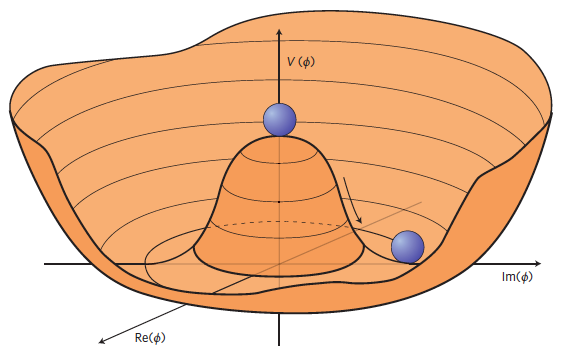
\includegraphics[width=0.5\textwidth]{fig/higgspotential}
    \caption{The Mexican hat potential for the scalar Higgs boson. The
    symmetric state at $\phi=0$ is spontaneously broken and a new vacuum state
is chosen in a random direction. For a particular choice of ground state, the
low-energy excitations look like a massive scalar field in addition to a
massless Goldstone field. After a local gauge transformation, a mass term
for the vector bosons becomes visible in the lagrangian \cite{mexhat}.}
    \label{fig:mexhat}
\end{figure}

\subsection{Higgs decay and production}
\label{sec:bg}
Apart from maybe neutrinos, whose mass-generating principle is not yet known,
the Higgs boson couples and thus can decay to all SM particles. However, the
top quark is too massive to be a real decay product of the Higgs boson. Since
the Higgs couples proportionally to the mass of the particle, decays to heavier
particles are favoured. The largest decay channels are to bottom quarks
(57.8\%), W bosons (21.6\%) and tau leptons (6,4\%). Even though photons are
massless, they can be the result of a Higgs decay by means of virtual top quark
loops. The Branching ratio to photons is only 0.2\%.
At the LHC, the two most important Higgs production mechanisms are gluon-gluon
fusion and vector boson fusion \cite[p.\;490f]{thomson}. Although the former
has a significantly higher cross section (10$\times$ higher), vector boson fusion is more
practical, since the virtual top quark loops lead to QCD radiation from the
colour field that makes identifying a Higgs decay more challenging.\\
Since Higgs decays are hard to separate from the usual multi jet events at the
LHC, decay channels with distinctive final state topologies are favoured. These
include $H\rightarrow\gamma\gamma$ and $H\rightarrow ZZ^*\rightarrow
l^+l^-l^+l^-$. In this lab, the four lepton states are the most important. 
These have to be separated from other four lepton state processes such as
$t\bar t$ pair production, where each of the two top quarks sends out two W bosons, changing
flavour each time. These W's can then each decay into a lepton neutrino pair.
Another background four-lepton process is the combination of a Z decaying into
two leptons together with a $b\bar b$ pair, each decaying into a lepton,
neutrino pair via a W boson.




\section{Experimental setup and methods}
\label{sec:setup}
\subsection{ATLAS detector}
\begin{figure}[h!]
    \centering
    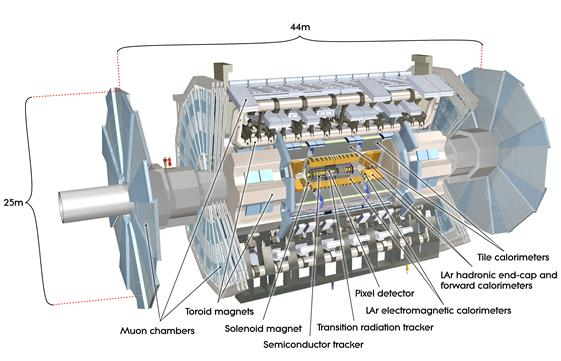
\includegraphics[width=0.7\textwidth]{fig/atlas}
\caption{Cross section of the ATLAS detector \cite{atlas}}
    \label{fig:atlas}
\end{figure}
The ATLAS detector is one of four major experiments at the Large Hadron
Collider at Cern. It is built for general purpose experiments with
proton-proton collisions. Its main goal has been the detection of the Higgs
boson, tests of the Standard Model and search for new physics beyond the SM,
such as supersymmetry and extra dimensions.
The detector itself consists of a inner detector, a calorimeter and the muon
spectrometer. The inner detector is a collection of different systems like a
pixel detector and semiconductor tracker for measuring the direction, momentum
and charge of charged particles, which are brought on a circular path by large
magnetic fields parallel to the beam axis. The transition radiation tracker
additionally provides information on which type of particle was detected. Next,
the electromagnetic and hadronic calorimeters are designed to absorb as much
energy of the produced particles as possible. This yields the direction and
energy of particles as well as a means to distinguish leptons from hadrons. 
Muons however, being a weakly ionising particle mostly flies through these
calorimeters. Therefore, the largest part of the detector is the muon
spectrometer, which is there to give very precise measurements of the muon
momentum.\\
The parameters that are used to describe particle trajectories and
energy-momentum are
\begin{itemize}
    \item The azimuthal angle $\phi$
    \item The pseudorapidity $\eta=-\ln\left[ \tan \left( \frac{\theta}{2}
        \right) \right]$
    \item the $z$ coordinate along the beam axis
    \item the transverse momentum $p_T=\sqrt{p_x^2+p_y^2}$
        
\end{itemize}


\subsection{ATLAS event display}
ATLANTIS, the ATLAS event display is used to depict the detector responses for
various decay processes graphically to get a feel for the different decay
topologies. From a view along the z-axis as well as from a side view, the tracks
in the inner detector and the muon spectrometer, as well as the showers in both
calorimeters can be seen. Additional information on the measured quantities can
be obtained upon selection of these features.
\begin{figure}[]
    \centering
        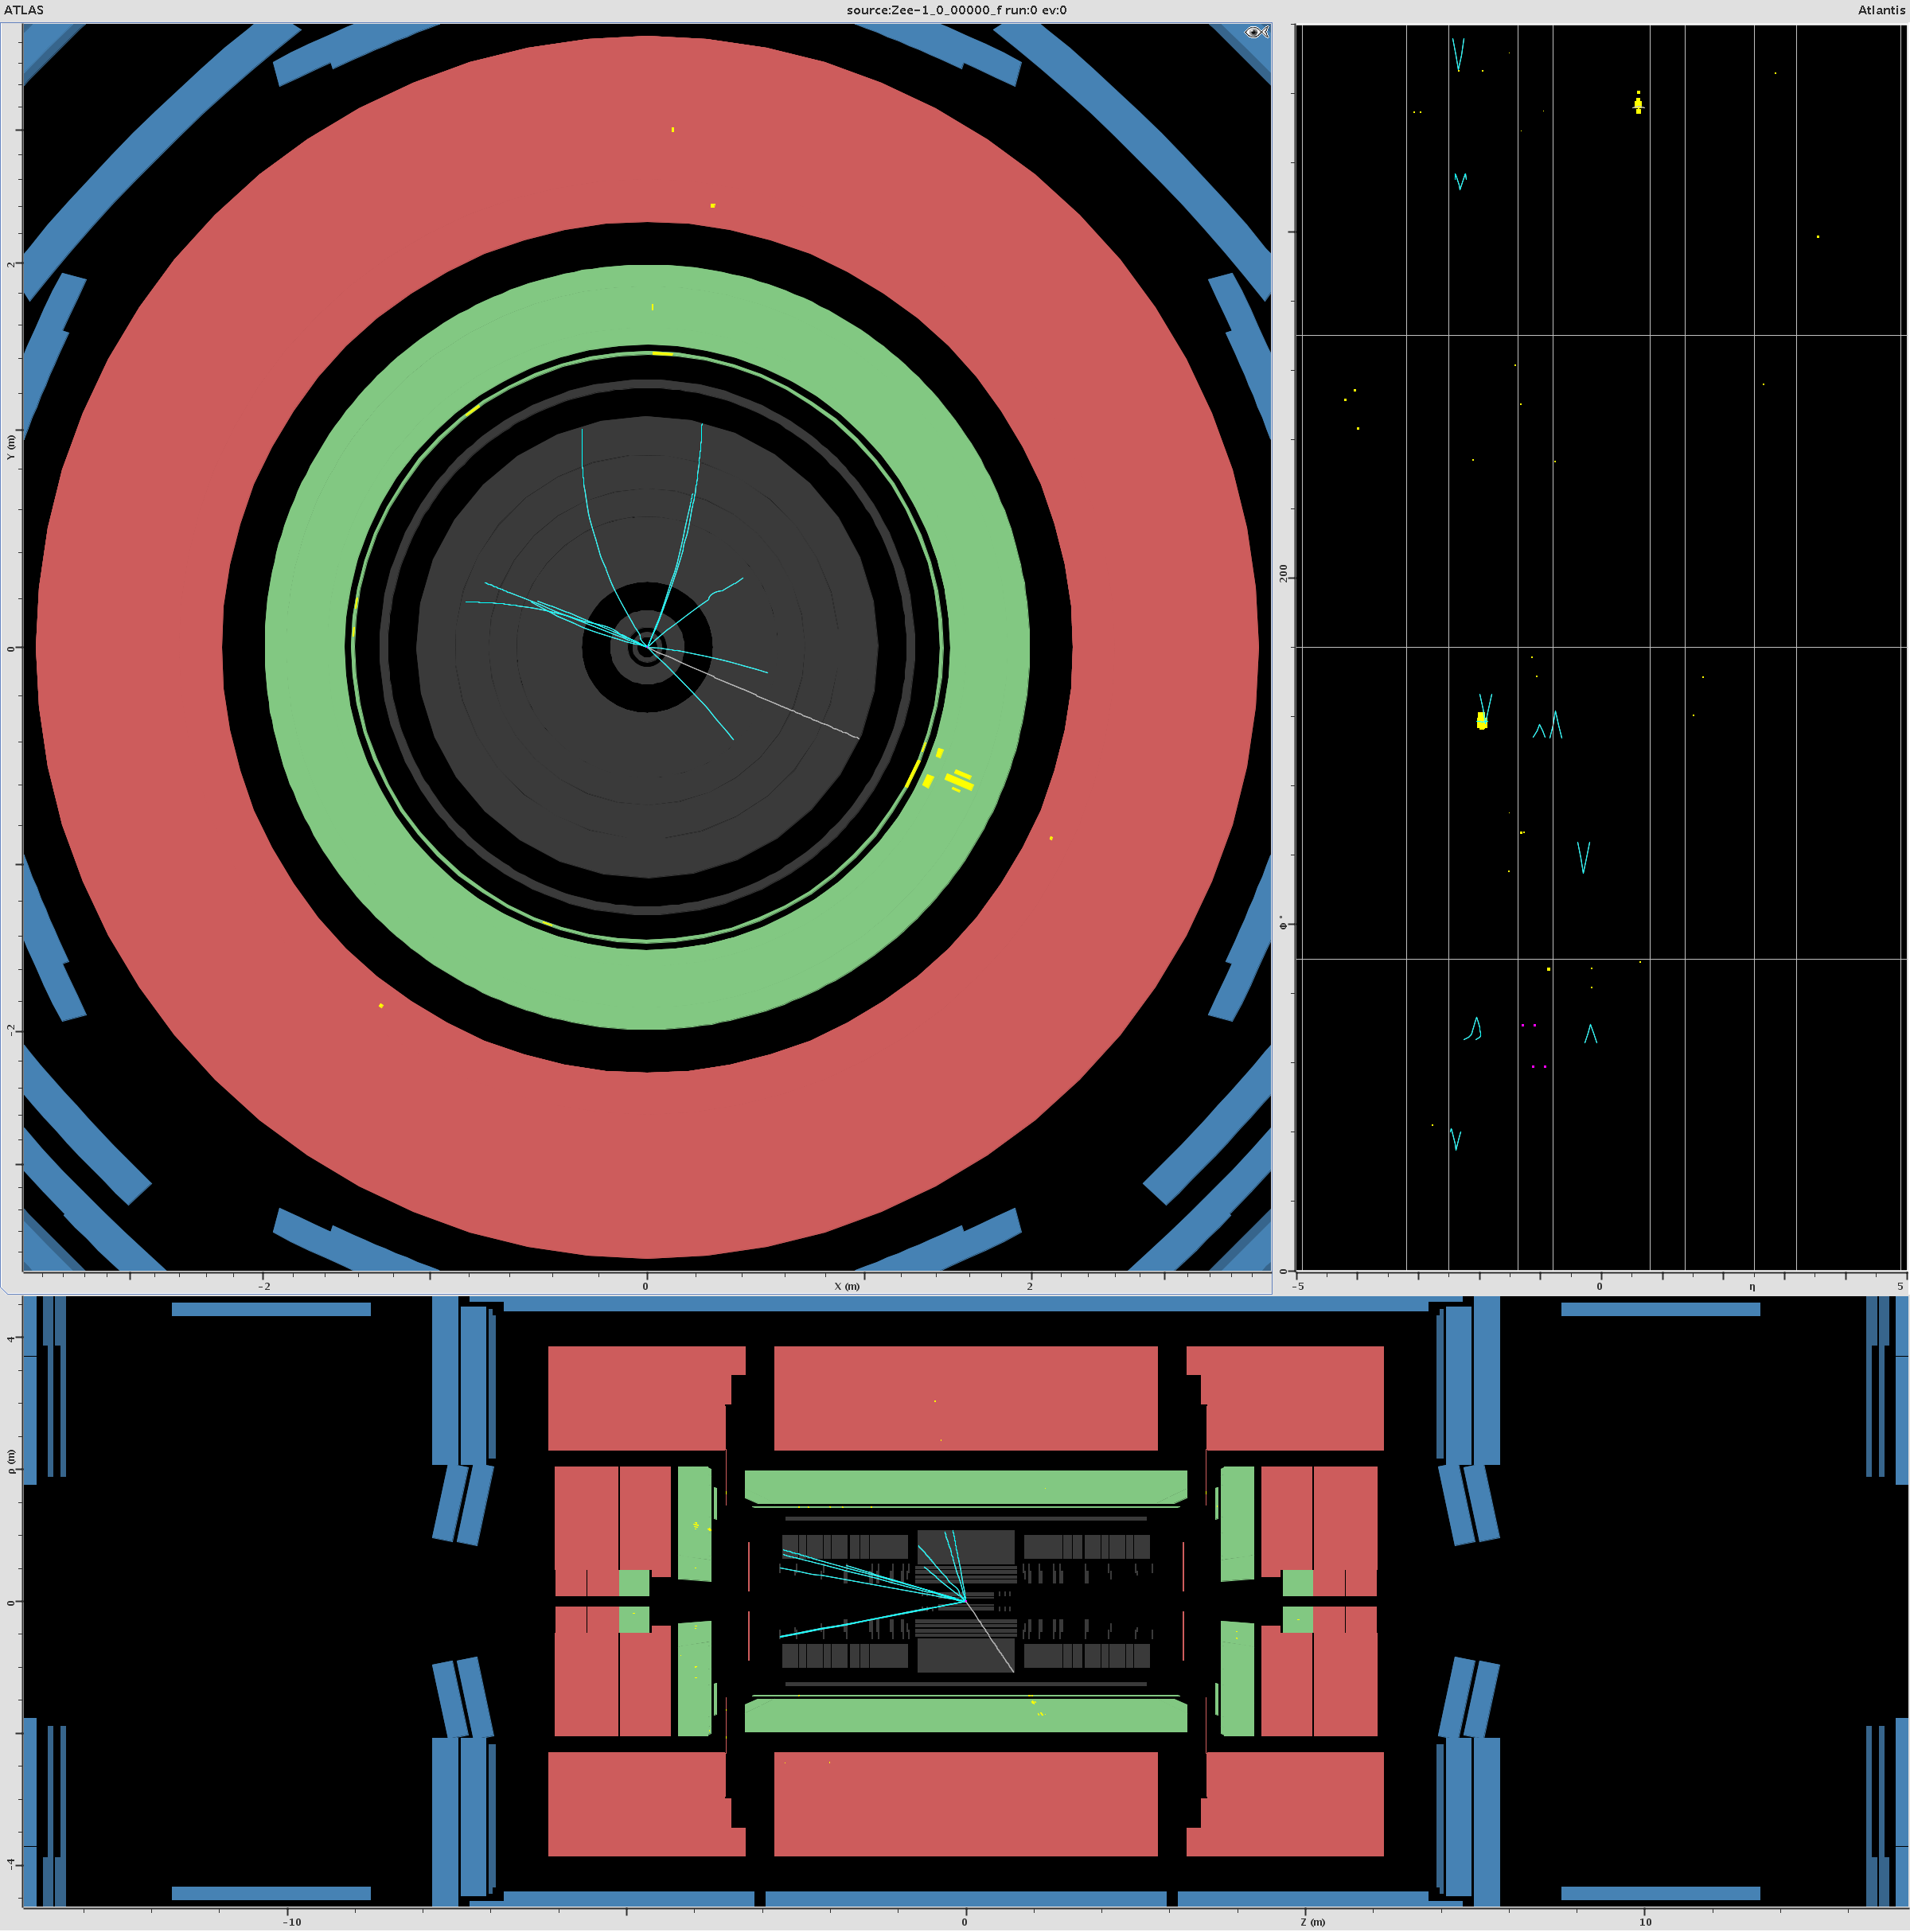
\includegraphics[width=0.6\textwidth]{fig/Zee}
    \caption{Z$\rightarrow e^+e^-$ decay viewed in ATLANTIS}
    \label{fig:atlantis}
\end{figure}




\section{Analysis}
\label{sec:analysis}
\subsection{Detector Responses to specific processes}
For this part of the lab, simulated data for single particle detection are
evaluated using ATLANTIS. Of course, such a single particle process is highly
unphysical because of background and additional decay products.
\subsubsection{Electron, $e^-$}
For a single electron, a well-defined single track in the inner detector is
observed. Its curvature is due to the electric charge and the magnets which
force the particle on a curved trajectory. Aligning with the track is a small
deposit in the electromagnetic calorimeter right behind the inner detector.
There, electrons radiate photons that lead to electron-positron pair
production. This leads to a shower.\\
In rare cases, the tracks in the inner detector are not consistent with the
showers in the calorimeter. Therefore it is clear that reconstruction errors
are still possible in such simple cases. There is also a possibility that an
electron emits a photon before reaching the calorimeter.

\subsubsection{Muon,$ \mu^-$}
Muons are especially easy to identify by a long track in the muon spectrometer
that is consistent with a track in the inner detector. As they have a mass of
around 100\;GeV, they are minimally ionising, meaning that they pass through
both calorimeters with virtually no trace. This is the reason for the large
muon spectrometers in the first place.

\subsubsection{Photon, $\gamma$}
Photons leave mostly no tracks inside the spectrometers since they are electrically
neutral and don't typically ionize. However, there is the possibility of
electromagnetic radiation leaving ionization tracks in the inner detector which
leads to a possible misidentification as electrons. The calorimeter responses
are equivalent to those of an electron.

\subsubsection{Tau, $\tau$}
Proper identification of tau leptons is very tricky as it is not directly
observable owing to its very short lifetime. Only its decay products are
visible in the detector. It decays via the weak interaction, always producing
at least one tau-neutrino in addition to mostly either an electron-neutrino or
muon-neutrino pair, or a pion. The latter subsequently decay
mostly into $\mu\nu_\mu$ pairs in the case for charged pions or two photons in
the case of neutral pions.
Reconstructing taus is therefore very challenging, due to the plethora of
possible decay products, as well as the neutrinos, which are invisible to the
detector and have to be inferred from indirect measurements of the missing
transverse momentum.\\
The observed tau events are often similar to either the electron or muon case.
But also different topologies are possible, e.g. three tracks and small
deposits in the hadronic calorimeter in addition to deposits in the
electromagnetic calorimeter. Rarely, a muon track is observed in the muon
spectrometer owing to the decay of a neutral pion.

\subsubsection{Dijets}
The dijet events consist of a large amount of tracks and energy deposits.
The strong force does not allow for the free propagation of single quarks or
gluons. Instead, quarks and gluons hadronise creating additional quark pairs
and gluons. This results in cone shaped tracks and deposits in the
calorimeters. These hadron showers -also referred to as jets- are typical in
proton proton collisions and form a large part of the background. Typically two
jets will stand out from the rest in their high energy, leaving the biggest
deposit in the calorimeters. Aditionally, they are minimally
curved in the inner detector due to their large momentum. These two jets are
therefore identified as coming directly from the interactions of the partons
making up the original protons that collided. The rest of the jets originate
from low energy charged particles.

\subsection{Analysis of muon momenutm loss}
\begin{table}
  \centering
  \begin{tabular}{|c|c|c|c|c|c|c|}
  \hline
  Event&\multicolumn{2}{c|}{Inner Detector}&\multicolumn{2}{c|}{Muon Spectrometer}&\multicolumn{2}{c|}{Loss}\\
  &$p_{ID}$ [GeV]&$p_{T,ID}$ [GeV]&$p_{MS}$ [GeV]&$p_{T,MS}$
  [GeV]&$\Delta{{p}}$ [GeV]&$\Delta{{p}_{T}}$ [GeV]\\
  \hline
  1&$-85.28$&$-38.36\pm 1.016$&$-57.62$&$-25.72$&$27.66$&$12.64\pm 1.016$\\
  2&$43.40$&$33.17\pm 0.797$&$47.53$&$36.17$&$-4.13$&$-3.00\pm 0.797$\\
  3&$-241.37$&$-41.85\pm 3.633$&$-240.72$&$-41.67$&$0.65$&$0.18\pm 3.633$\\
  4&$48.89$&$41.96\pm 0.831$&$-48.47$&$41.26$&$0.42$&$0.70\pm 0.831$\\
  5&$-168.16$&$-53.66\pm 2.054$&$-181.32$&$-62.44$&$-13.6$&$-8.78\pm 2.054$\\
  6&$117.32$&$44.65\pm 1.388$&$100.26$&$38.01$&$17.06$&$6.64\pm 1.388$\\
  7&$-71.94$&$-57.39\pm 1.684$&$-68.66$&$-54.77$&$3.28$&$2.62\pm 1.684$\\
  8&$199.91$&$64.54\pm 2.677$&$203.14$&$66.99$&$-3.23$&$-2.45 \pm 2.677$\\
  9&$-57.84$&$-55.54\pm 1.150$&$-53.71$&$-51.16$&$4.13$&$4.38\pm 1.150$\\
  10&$-100.75$&$-37.79\pm 1.185$&$-97.81$&$-36.40$&$2.94$&$1.39\pm 1.185$\\
  11&$38.26$&$37.59\pm 0.653$&$38.18$&$37.48$&$0.08$&$0.11\pm 0.653$\\
  12&$-105.19$&$-59.88\pm 1.766$&$-112.38$&$-64.27$&$-7.19$&$-4.39\pm 1.766$\\
  13&$236.12$&$47.52\pm 3.324$&$267.31$&$53.73$&$-31.19$&$-6.21\pm 3.324$\\
  14&$-131.69$&$-43.88\pm 1.471$&$-129.21$&$-43.21$&$2.48$&$0.67\pm 1.471$\\
  15&$152.24$&$45.66\pm 1.844$&$161.39$&$48.37$&$-9.15$&$-2.71\pm 1.844$\\
  16&$-35.23$&$-33.65\pm 0.539$&$-35.88$&$-33.23$&$-0.65$&$0.42\pm 0.539$\\
  17&$54.19$&$52.80\pm 1.060$&$53.70$&$52.33$&$0.49$&$0.47\pm 1.060$\\
  18&$-84.75$&$-64.49\pm 2.515$&$-71.79$&$-55.02$&$12.96$&$9.47\pm 2.515$\\
  19&$104.26$&$47.56\pm 1.324$&$111.68$&$51.21$&$-7,42$&$-3.65\pm 1.324$\\
  20&$-184.01$&$-35.52\pm 2.24$&$-174.36$&$-33.96$&$9.65$&$1.56\pm 2.284$\\
  \hline
  \end{tabular}
  \caption{Momenta $p$, and transverse momenta $p_T$ for the first twenty
  events, measured both in the inner detector and the muon spectrometer. The
  difference between these $p_\text{loss}$, ${p_T}_\text{loss}$ is also shown.
  Negative losses indicate a gain in momentum after passing the calorimeters.}
  \label{tab:loss}
\end{table}

For the single muon dataset, both the momentum $p$ and the transverse momentum
$p_T$ are
read out using ATLANTIS for the first 20 events. Values are read out from the
inner detector (ID) and the muon spectrometer (MS). An uncertainty $\sigma$ is
also given for both values for the inner detector. Contrary to the multi
purpose inner detector, the uncertainty is assumed to be negligible for the
muon spectrometer, since its size allows for large tracks and therefore great
accuracy. Additionally the muon detector elements are specialized for muons.
The loss of (transverse) momentum
$\Delta{{p}_{(T)}}=|p_{(T)\text{ID}}|-|p_{(T)\text{MS}}|$ is
calculated. Uncertainty is propagated using the gaussian formula. The result is
shown in \cref{tab:loss}.
Interestingly, for 7 out of the 20 events, the muon spectrometer measured a
higher transverse momentum than the inner detector. This is furthermore not
consistent with the uncertainties from the inner detector.

The average loss of momentum is calculated with a weighted
average:
\begin{align}
    \bar p = (\sum \frac{p}{\sigma^2})/(\sum \frac{1}{\sigma^2}),\qquad \sigma_{\bar p} = \sqrt{1/(\sum \frac{1}{\sigma^2})}.
\end{align}
One obtains
\begin{align}
    \label{eq:resavg1}
    \bar{\Delta}{{p}_{T}}=(0.91\pm0.25)\;\text{GeV}.
\end{align}
In the assumption that negative momentum losses are unphysical and thus
ignoring them, one obtains instead:
\begin{align}
    \bar{\Delta}{{p}_{T}}=(2.12\pm0.28)\;\text{GeV}.
\end{align}

\subsection{Reconstruction of the $Z$ mass}
Simulated data from $Z\rightarrow e^+e^-$ events are analyzed using ATLANTIS.
Here, events with two distinct  high energy deposits in the calorimeter could
be found. These are assumed to be the electron and positron respectively. An
example of such an event is seen in \cref{fig:atlantis}. By selecting the
tracks or the calorimeter deposits manually, various parameters can be read
off. For the tracks in the inner detector, the azimuthal angle $\phi$, the
pseudorapidity $\eta$ and both the transverse and total momentum $P_{(T)}$ were
noted. From the electromagnetic calorimeter the total and transverse energy
$E_{(T)}$ was taken. The values are summed up in \cref{tab:zrec}.

The invariant mass of the Z boson can be written as the four-vector
norm-squared of the sum of the energy momentum vectors of both leptons \cite{kinematics}:
\begin{align}
    M_Z^2=(p_1^\mu+p_2^\mu)^2&=m_1^2+m_2^2+2[E_1
    E_2-\vec{p_1}\cdot\vec{p_2}]\\&=m_1^2+m_2^2+2[E_1
    E_2-(E_{T_1}E_{T_2}(\beta_{T_1}\beta_{T_2}\cos(\Delta\phi)+\sinh(y_1)\sinh(y_2)\;))].
\end{align}
In the second line, the three-vector scalar product has been expanded in terms
of the rapidity $y$, the azimuthal angle $\phi$ and the transverse (rel.)
velocity $\beta_T$. For a highly relativistic electron with $p=50\;$GeV, the rest mass can be
ignored, thus setting $m_1=m_2=0,\;E_{(T)}=p_{(T)},\;\beta_{(T)}=1,\;\eta=y$,
which reduces the Z mass formula to
\begin{align}
    \label{eq:zmass}
    M_Z=\sqrt{2E_{T_1}E_{T_2}(\cosh(\Delta y)-cos(\Delta\phi))}.
\end{align}
Errors are calculated by the usual gaussian error propagation. However, it has
to be kept in mind that the only uncertainty given by the detector was that of
the transverse momentum measured in the inner detector and the pseudorapidity.
A large amount of uncertainty can also be attributed to the selection of the
energy deposits in the calorimeter, which was done manually. However such an
error has not been included.
The final results are shown in \cref{tab:zres}. Clearly, for event $b)$, the
result does not conform to the literature value and the total momentum of the
second lepton does not have the same order of magnitude as the calorimeter
energy.
\begin{table}
\centering
\begin{tabular}{|c c|c|c|c|c|c|c|}
\hline
& & \multicolumn{4}{c|}{Inner Detector}&\multicolumn{2}{c|}{EM
Calorimeter}\\
& &$\phi$&$\eta$&$p_T$ [GeV]&$p$ [GeV]&$E$ [GeV]&$E_T$
[GeV]\\
\hline
\multirow{2}{*}{a)}&$e_1$&$5.860$&$0.610\pm
0.001$&$-19.20\pm 0.297$&$-22.88$&$22.2$&$18.6$\\
&$e_2$&$2.771$&$-1.953\pm 0.001$&$25.38\pm
0.860$&$91.29$&$88.6$&$24.6$\\
\hline
\multirow{2}{*}{b)}&$e_1$&$5.187$&$2.193\pm
0.000$&$-44.75\pm 2.673$&$-202.97$&$175.4$&$38.6$\\
&$e_2$&$1.485$&$2.432\pm 0.002$&$3.72\pm
0.180$&$21.84$&$259$&$45.5$\\
\hline
\multirow{2}{*}{c)}&$e_1$&$0.826$&$-0.610\pm
0.001$&$-41.69\pm
0.752$&$49.69$&$49.9$&$42.0$\\
&$e_2$&$3.926$&$-0.983\pm 0.001$&$39.98\pm
1.581$&$60.92$&$58.0$&$38.4$\\
\hline
\end{tabular}
\caption{ATLAS Parameters for both
leptons in three $Z\rightarrow e^+
e^-$ events.}
\label{tab:zrec}
\end{table}

\begin{table}
\centering
\begin{tabular}{|c|c|c|}
\hline
& $M_Z$ [GeV] from ID&
$M_Z$ [GeV] from EM
Cal.\\
\hline
a)&$85.7\pm
1.6$&$83.2\pm
0.1$\\
\hline
b)&$28.8\pm
1.0$&$71.8\pm
0.1$\\
  \hline
    c)&
    $83.1\pm
    1.9$&$80.0\pm
    0.1$\\
      \hline
        \end{tabular}
          \caption{Reconstructed
          $Z$
          boson
          mass,
          $M_Z$,
          from
          three
          $Z\rightarrow
          e^+e^-$
          events
          with
          the
          transverse
          energy
          obtained
          from
          either
          the
          inner
          detector
          or
          the
          EM
          calorimeter.}
            \label{tab:zres}
        \end{table}
\subsection{Determination of cut criteria for $ZZ$ selection}
The aim of this part of the lab is the development of cut criteria to extract
the signal of $ZZ\rightarrow llll$ processes from the background of the $t\bar
t$ pair production and the $Z b\bar b$ background summarized in \cref{sec:bg}.
The datasets used are all monte-carlo simulations. The $Z^0$ pair signal
corresponds to an integrated luminosity of 400\;fb$^{-1}$, while all other
datasets correspond to $140$\;fb$^{-1}$. Different event parameter
distributions are plotted for both signal and background to determine which
parameters have a large amount of signal events and a small amount of
background events, or vice-versa. Because all background processes lead
to additional quarks produced with the four leptons, the jet properties of the
events is used to extract the signal. First, the number of jets per event is
shown in \cref{fig:cut1}. As expected, the background processes have a larger
number of jets. Thus, a cut requiring
\begin{align}
n_{\text{jets}}\leq2 
\label{eq:cut1}
\end{align}
is chosen. Furthermore, since the quarks are produced alongside the leptons, a
larger amount of energy deposit noise around the leptons is expected.
\cref{fig:cut2,fig:cut3} show this calorimeter noise $et_{iso}$ around both the most and
least energetic lepton. For the intermediate leptons, the plots look similar.
Background processes have a larger amount of noise, leading to the cut
condition 
\begin{align}
    et_{iso}\leq5\;\text{GeV.}
\label{eq:cut2}
\end{align}
Additional parameters such as the missing transverse energy were probed but did
not lead to a better reconstruction of the signal.
The amount of signal and background events before and after the cuts are
summarized in \cref{tab:cutresults}.
\begin{figure}[h!]
    \begin{center}
        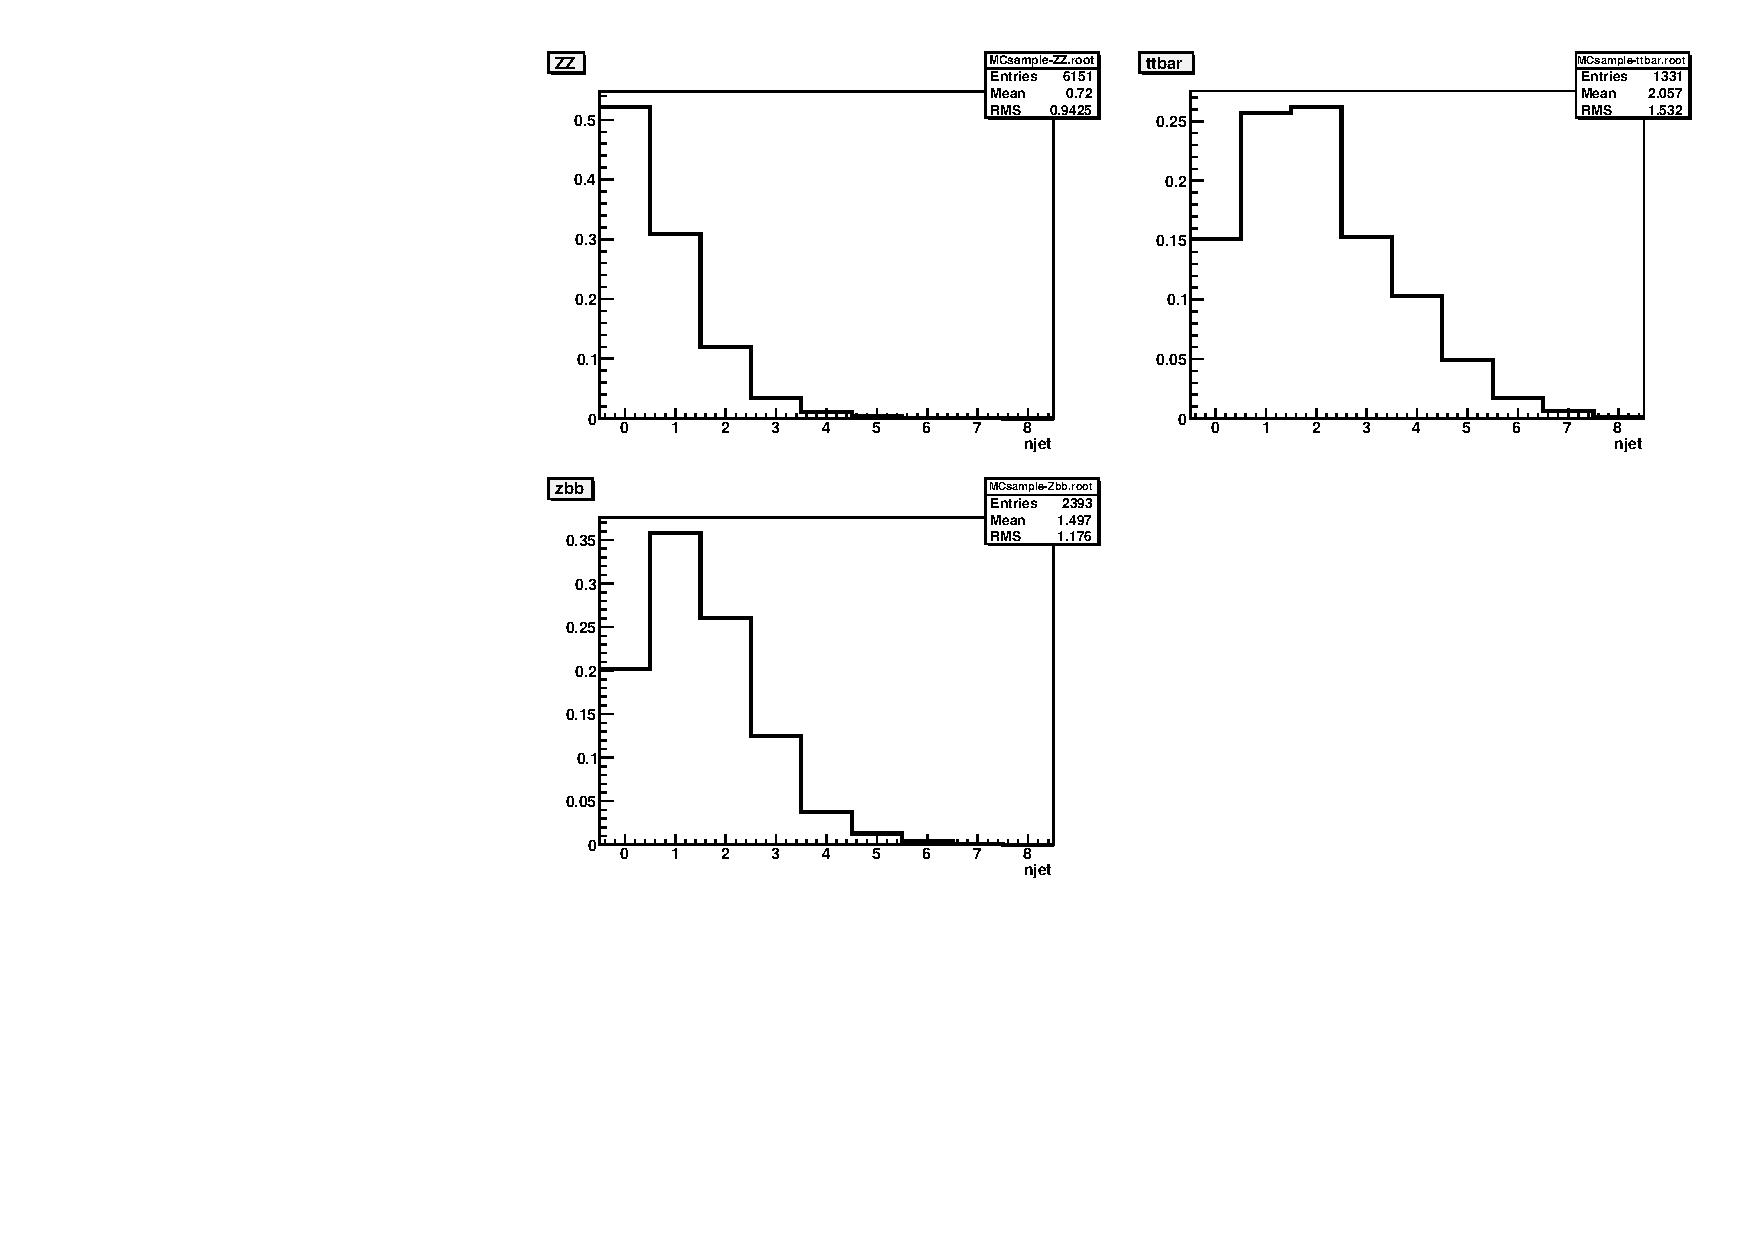
\includegraphics[width=0.7\textwidth]{ZZ/njets_uncut}
    \end{center}
    \caption{Number of jets for the $ZZ$ signal and the $t\bar t$ and $Zbb$
    monte carlo data.}
    \label{fig:cut1}
\end{figure}
\begin{figure}[h!]
    \begin{center}
        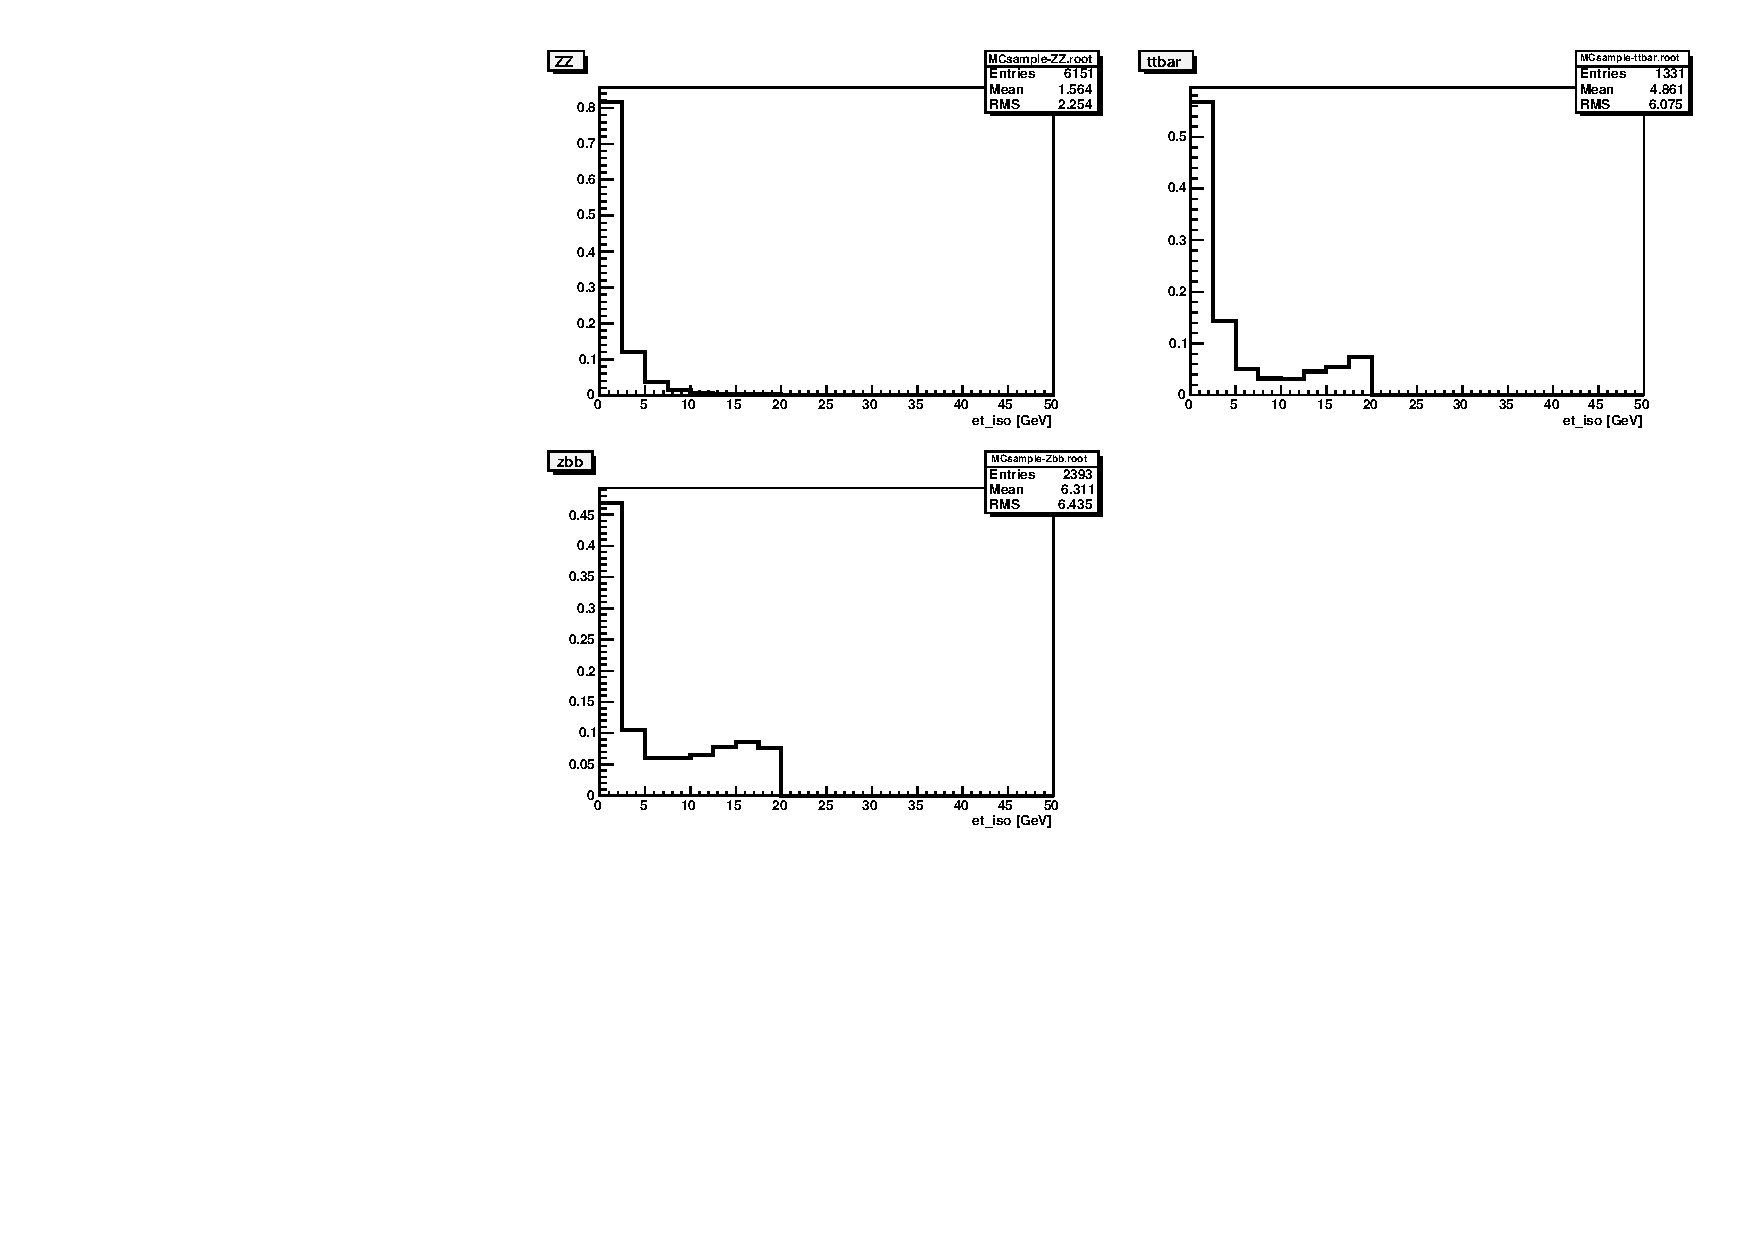
\includegraphics[width=0.7\textwidth]{ZZ/etiso1_uncut}
    \end{center}
    \caption{Calorimeter energy deposit around the most energetic lepton for
    the $ZZ$ signal and the $t\bar t$ and $Zbb$
    monte carlo data.}
    \label{fig:cut2}
\end{figure}
\begin{figure}[h!]
    \begin{center}
        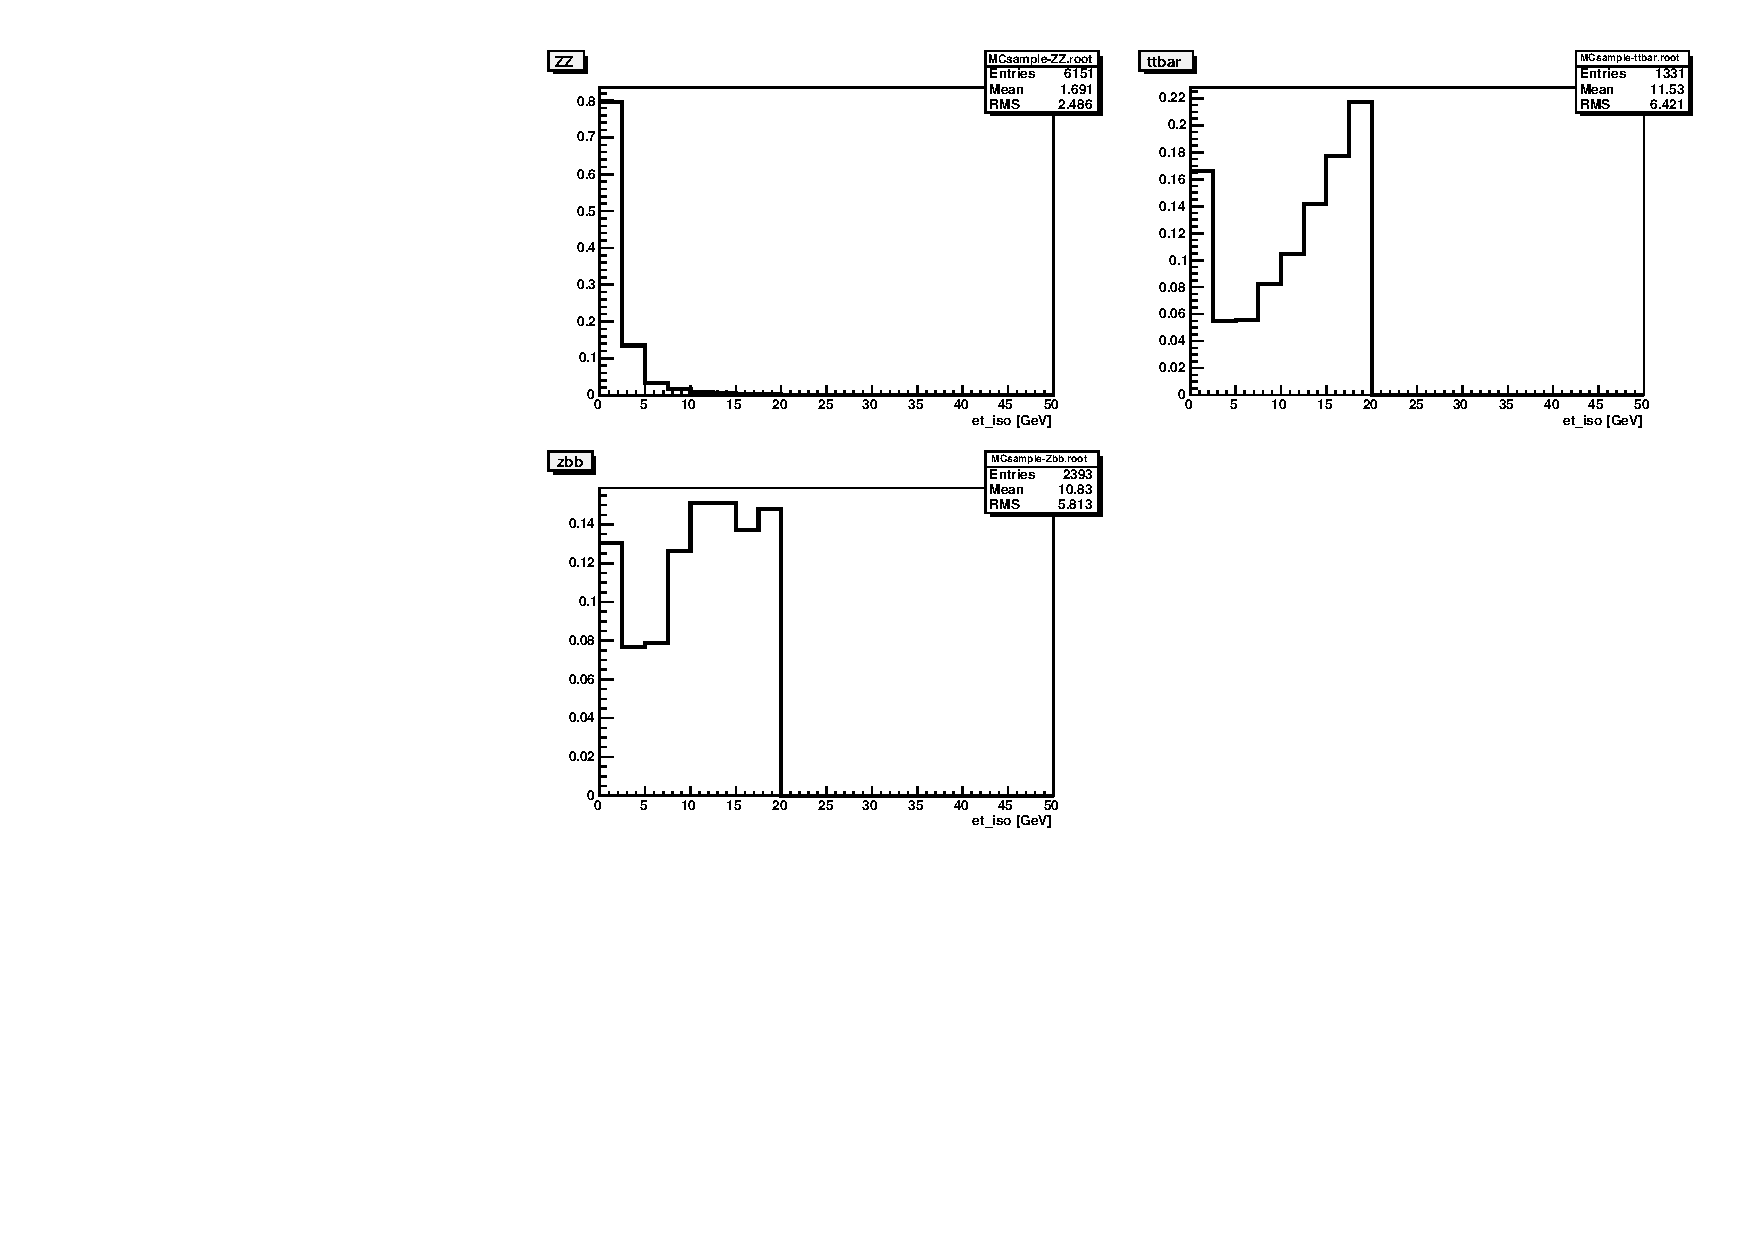
\includegraphics[width=0.7\textwidth]{ZZ/etiso4_uncut}
    \end{center}
    \caption{Calorimeter energy deposit around the least energetic lepton for
    the $ZZ$ signal and the $t\bar t$ and $Zbb$
    monte carlo data.}
    \label{fig:cut3}
\end{figure}

\subsection{Mystery $ZZ$ production threshold}
With the cuts above in place, a simulated ``mystery'' data set with an
integrated luminosity of 100\;fb$^{-1}$is investigated with respect to $ZZ$
pairs. A $Z$ boson is defined as a real one, if its mass is within two decay
withs $2\Gamma_Z=4.99\;$GeV around the nominal $Z$ mass $m_Z=91.19$
\cite{pdataz}. It can now be counted, whether the two $Z$ bosons produced are
both real $(ZZ)$, both virtual $(Z^*Z^*)$ or mixed $(ZZ^{*})$. To ensure that
the two leptons belonging to a particular $Z$ boson are identified correctly,
only the datasets with 2 electrons and 2 muons are used.
If the invariant mass of all four leptons is greater or equal to twice the $Z$
mass, the threshold is reached. This can be seen from
\begin{align}
    \label{eq:threshhold}
    M_{4l}=(\sum_{i=1}^4p_i^\mu)^2&=(p_1^\mu+p_2^\mu)^2+(p_3^\mu+p_4^\mu)^2+2(p_1^{\mu}+p_2^{\mu})(p_{3,\mu}+p_{4,\mu})\\
    &=2M_Z+2(p_1^{\mu}+p_2^{\mu})(p_{3,\mu}+p_{4,\mu})\geq2M_Z,
\end{align}
with lepton 1 and 2 originating from one $Z$ and 3 and 4 originating from the
other. The counting results are summed up in \cref{tab:ZZcount}.







\begin{table}
\centering
\begin{tabular}{|c|c|c|}
\hline
Process& Events before cut& Events after cut\\
\hline
$ZZ$ (sig)&$6151$&$4561$\\
\hline
$Zb\bar b$ (bkg)& $2393$&$17$\\
\hline
$t\bar t$ (bkg)&$1331$&$0$\\
\hline
\end{tabular}
\caption{Number of events before and after
application of the cut criteria detailed
above on the signal and background
processes.}
\label{tab:cutresults}
\end{table}
\begin{table}
\centering
\begin{tabular}{|c|c|c|}
\hline
& Above Threshold& Below
Threshold\\
\hline
$ZZ$&$934$&$13$\\
\hline
$ZZ^*$& $1553$&$319$\\
\hline
$Z^*Z^*$&$476$&$162$\\
\hline
\end{tabular}
\caption{Number
of events
above and
below the
production
threshold,
on-shell
($ZZ$),
off-shell
($Z^*Z^*$),
and mixed
($ZZ^*$)
discovered in
the provided
mystery
datasets.}
\label{tab:ZZcount}
\end{table}

\subsection{Higgs Boson and New Physics}
Here, three ``mystery'' data sets containing new physics and a simulated
standard model ATLAS data set are analyzed.
First, new physics is searched in the mystery data. Several variable
distribution were plotted against another to find differences in the four data
sets. After trying out various variables, it was found that a selection of
\begin{itemize}
    \item Missing transverse energy $etmis\geq100$\;GeV
    \item Calorimeter noise around each lepton $et_{iso}\leq10\;$GeV
\end{itemize}
left around $10\%$ of the events in mystery data set 2, while all other data
sets saw a reduction in events to 1\% (ATLAS) and 3\% (mystery 3 and 4) of the
initial events. The cut variable distribution are shown in
\cref{fig:myst1,fig:myst2,fig:myst3}, while the final invariant mass distribution after
the cuts are shown in \cref{fig:myst4}.
\begin{figure}[]
    \begin{center}
        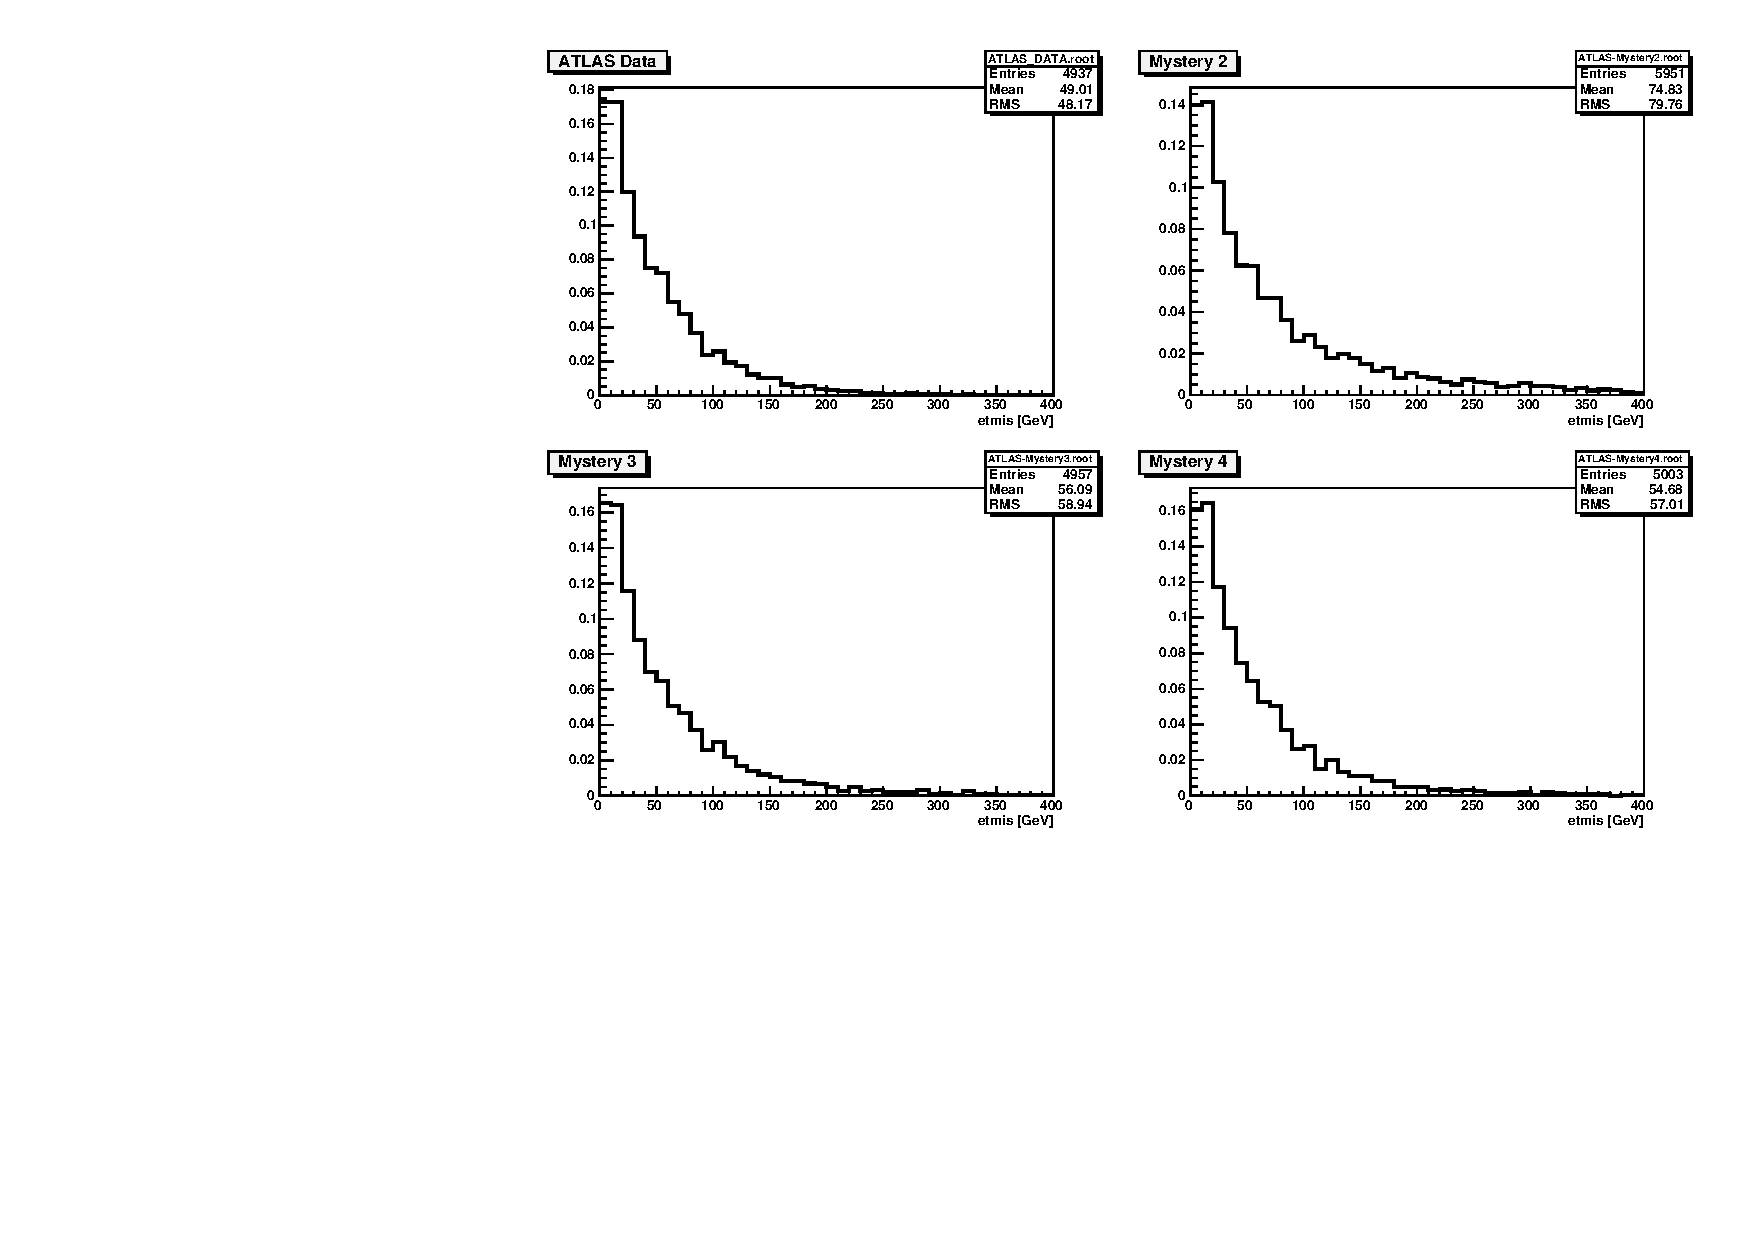
\includegraphics[width=0.8\textwidth]{ZZ/mystery_met_uncut.pdf}
    \end{center}
    \caption{Missing transverse energy distribution of the simulated ATLAS data and three mystery data sets.}
    \label{fig:myst1}
\end{figure}


\begin{figure}[]
    \begin{center}
        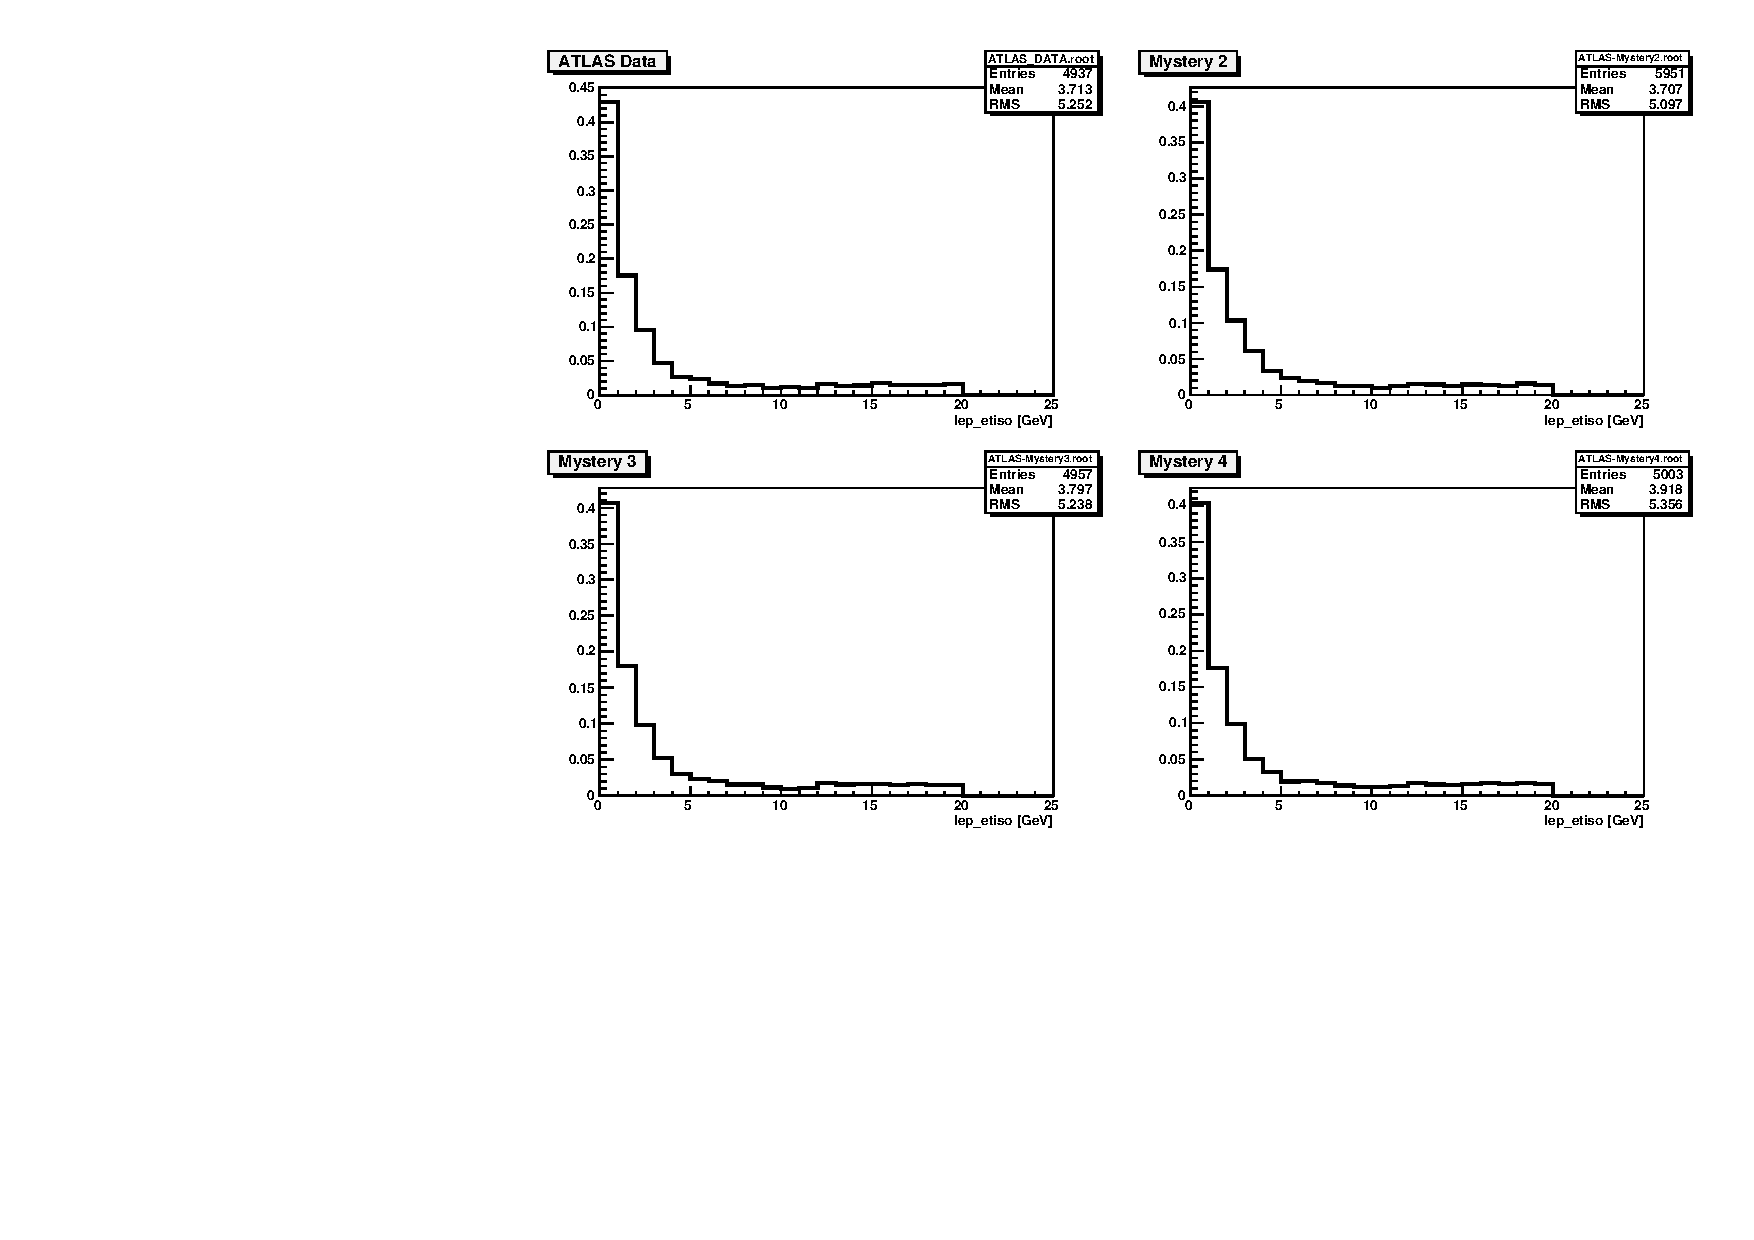
\includegraphics[width=0.8\textwidth]{ZZ/mystery_et_iso_1_uncut.pdf}
    \end{center}
    \caption{Calorimeter noise distribution for the most energetic lepton of the simulated ATLAS data and three mystery data sets.}
    \label{fig:myst2}
\end{figure}


\begin{figure}[]
    \begin{center}
        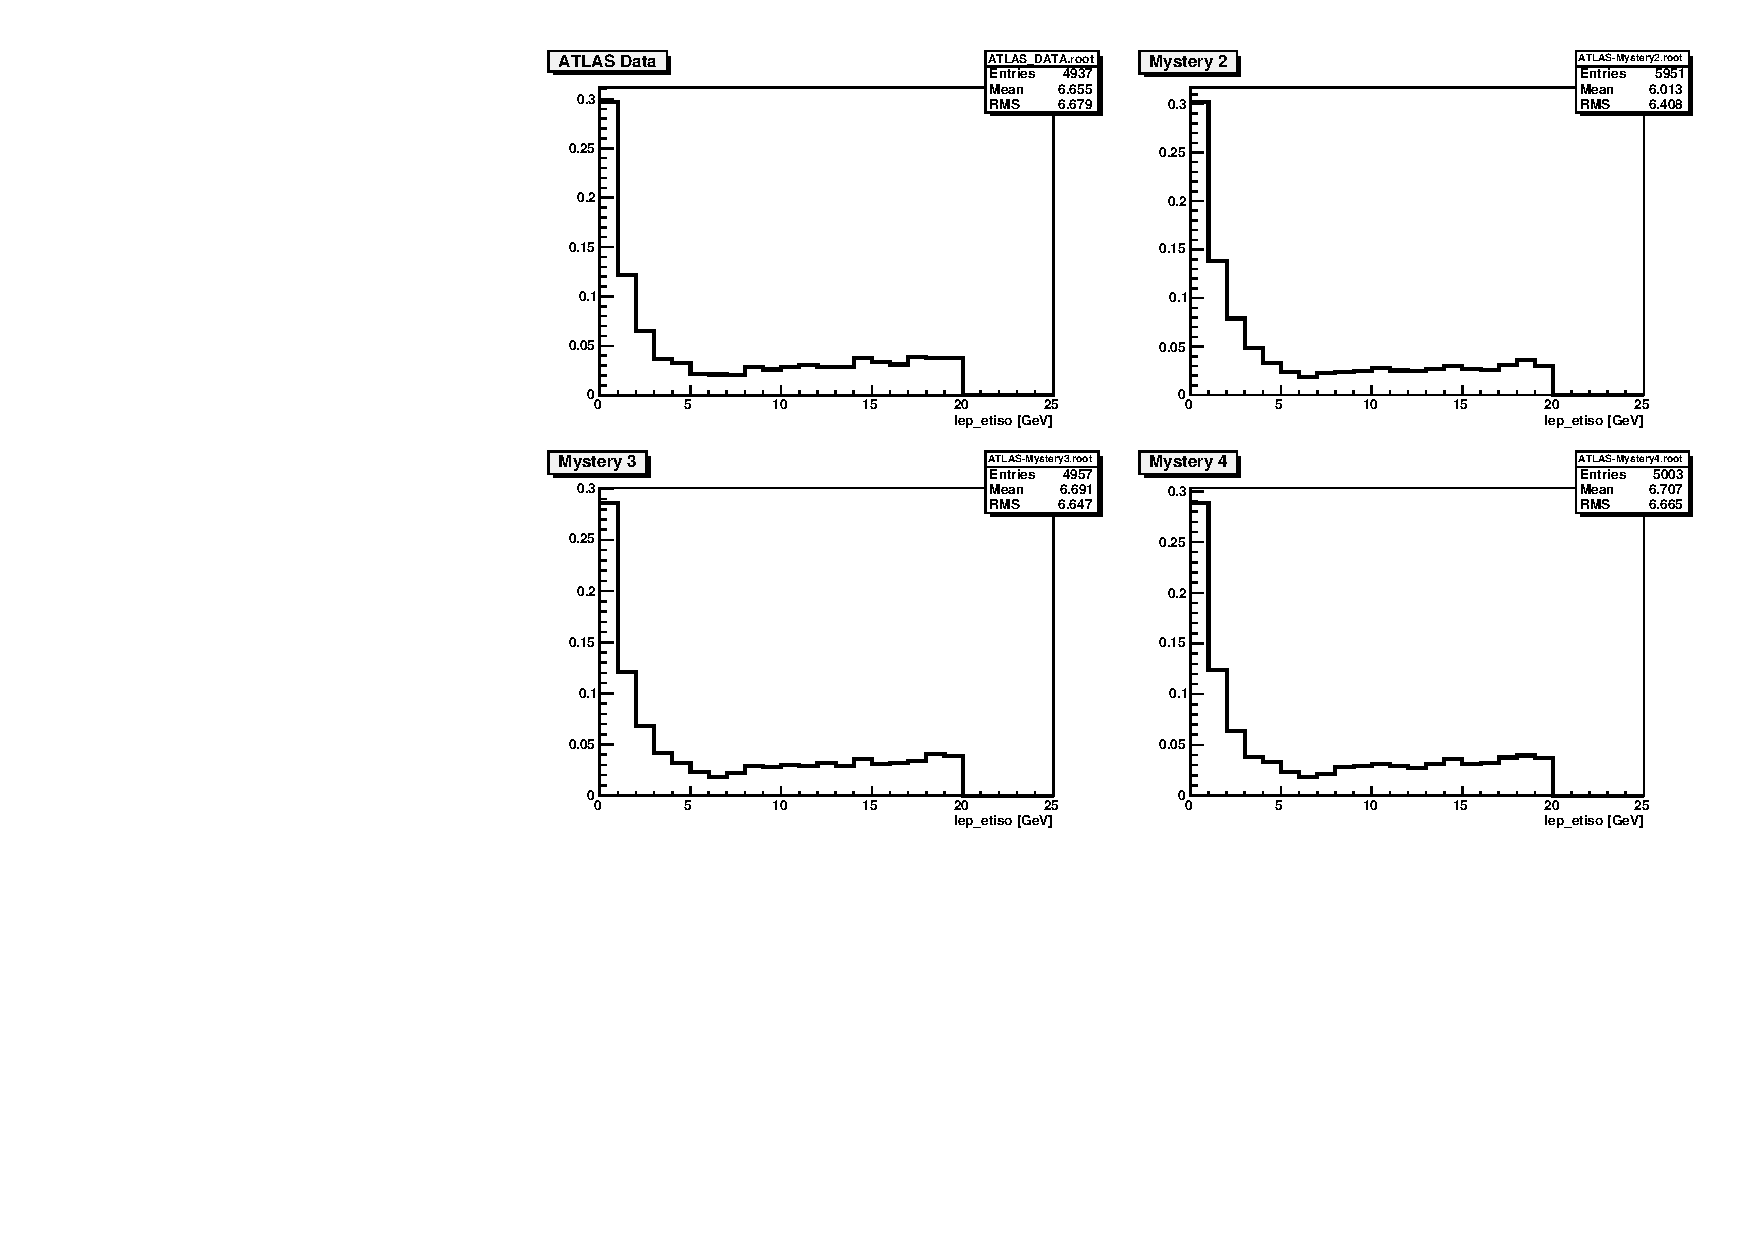
\includegraphics[width=0.8\textwidth]{ZZ/mystery_et_iso_4_uncut.pdf}
    \end{center}
    \caption{Calorimeter noise distribution for the least energetic lepton of the simulated ATLAS data and three mystery data sets.}
    \label{fig:myst3}
\end{figure}


\begin{figure}[]
    \begin{center}
        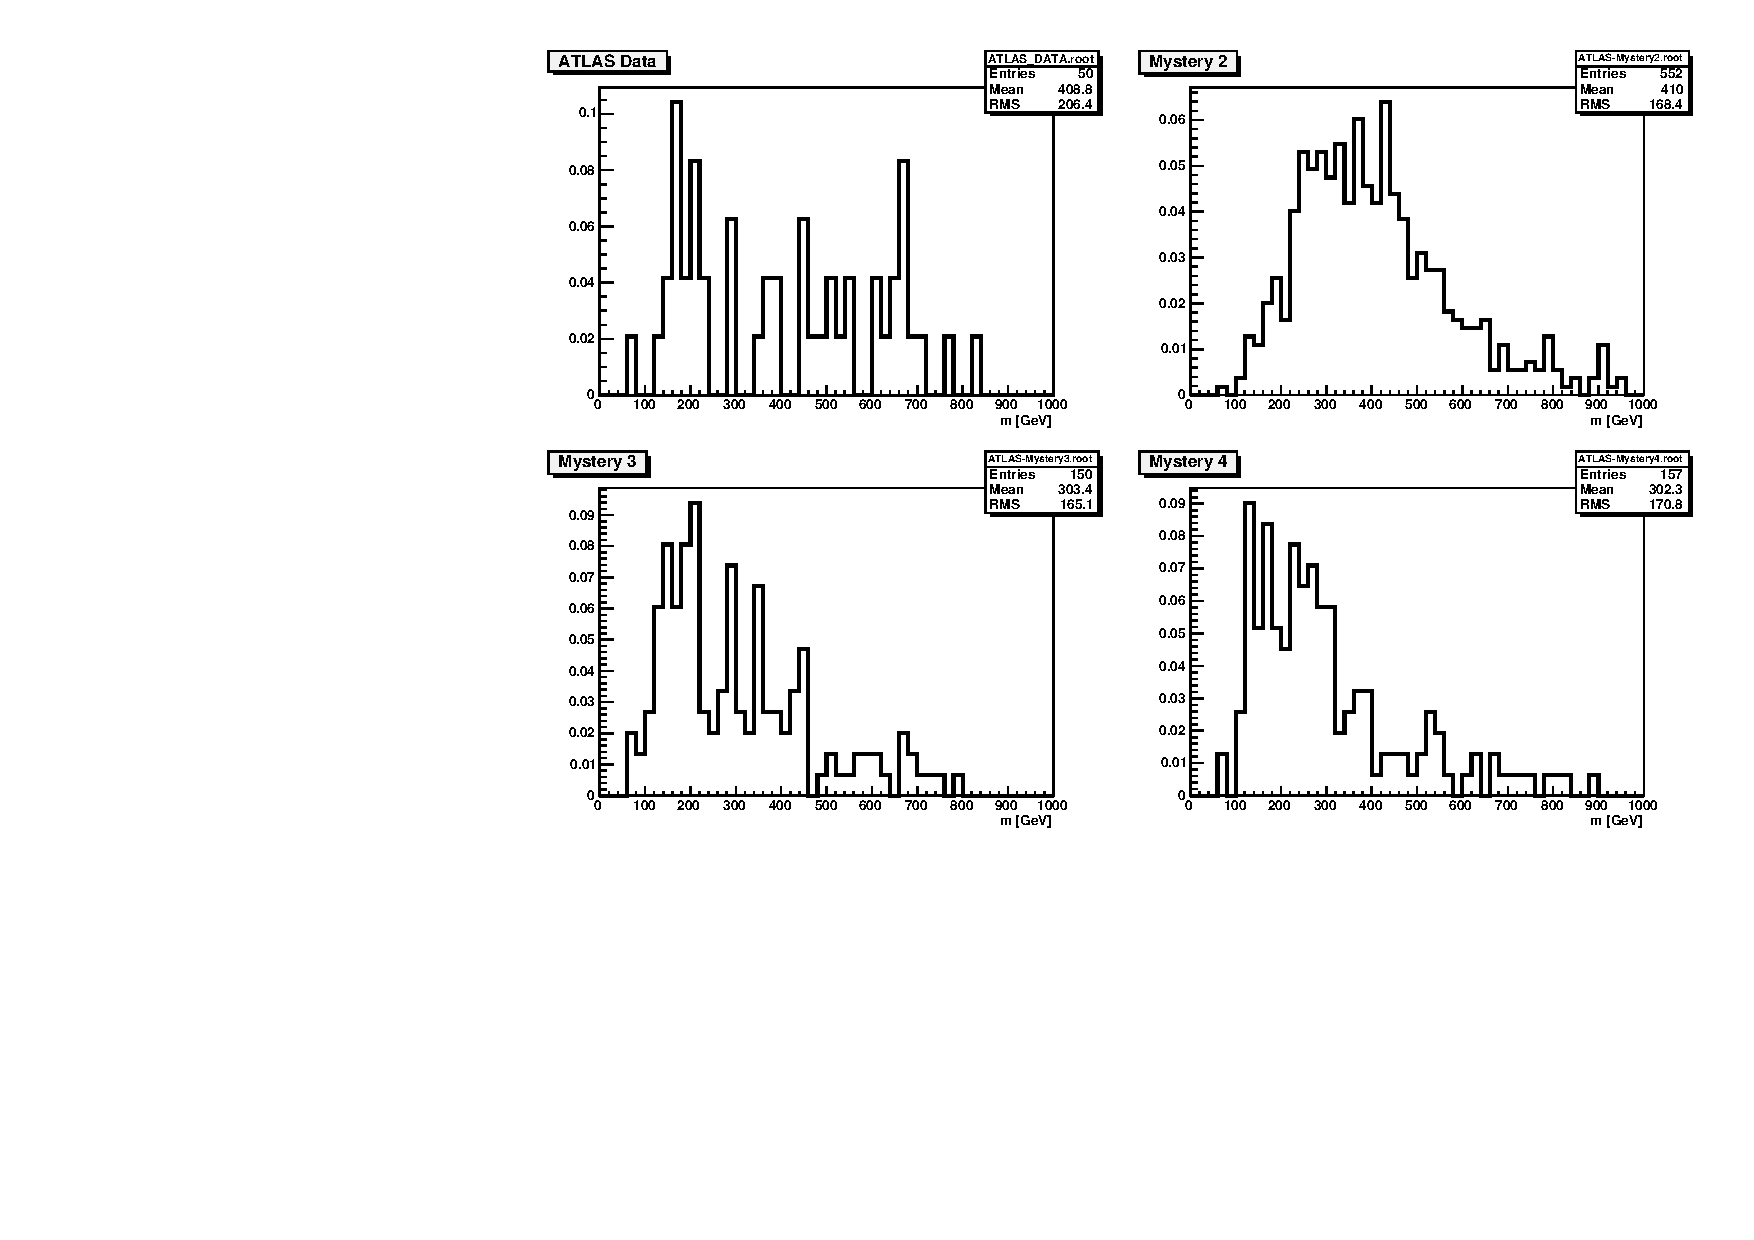
\includegraphics[width=0.8\textwidth]{ZZ/mystery_mass_cut.pdf}
    \end{center}
    \caption{Invariant mass distribution of the four leptons of the simulated ATLAS data and three mystery data sets.}
    \label{fig:myst4}
\end{figure}

Defining the mystery data set 2 as the signal, the significance is calculated
with \cite{signifikanz}
\begin{align}
    \label{eq:sig}
    Sig=\frac{S}{\sqrt{S+B}},
\end{align}
where S and B are the number of events in the signal and background
respectively, while the initial uncertainty is calculated with a poisson error
$\sigma_S=\sqrt S, \sigma_B=\sqrt B$. Thus, \cref{eq:sig} gives a measure of
the sensitivity that the signal is measured on top of the fluctuations of the
signal and background. The amount of signal events $S$ are calculated by
scaling the signal dataset to the luminosity of the ATLAS data of
$149\;$fb$^{-1}$ and then subtracting the ATLAS data.
This procedure results in a significance of the mystery2 signal of
\begin{align}
    \label{eq:singance}
    sig_{\text{ mystery2}}=26\pm1.
\end{align}

Finally, we want to isolate the Higgs boson from the ATLAS data simulation. For
this, cut criteria were developed similar to the above procedure. More
precisely, the $ZZ$, $Zb\bar b$ and $t\bar t$ processes from before have to be
discarded. The cut criteria used are:
\begin{itemize}
    \item Sum of the calorimeter transverse energy, $sumet\geq 700\;$GeV
    \item Missing transverse energy $et\_mis\geq200\;$GeV.
\end{itemize}
The mass distribution of the four leptons after cutting is shown in
\cref{fig:higgsmass}.
Calculating the significance analogously as before, one finally obtains
\begin{align}
    \label{eq:fastfertig}
    sig_{\text{ Higgs}}=2.6\pm1.1.
\end{align}
\begin{figure}[]
    \begin{center}
        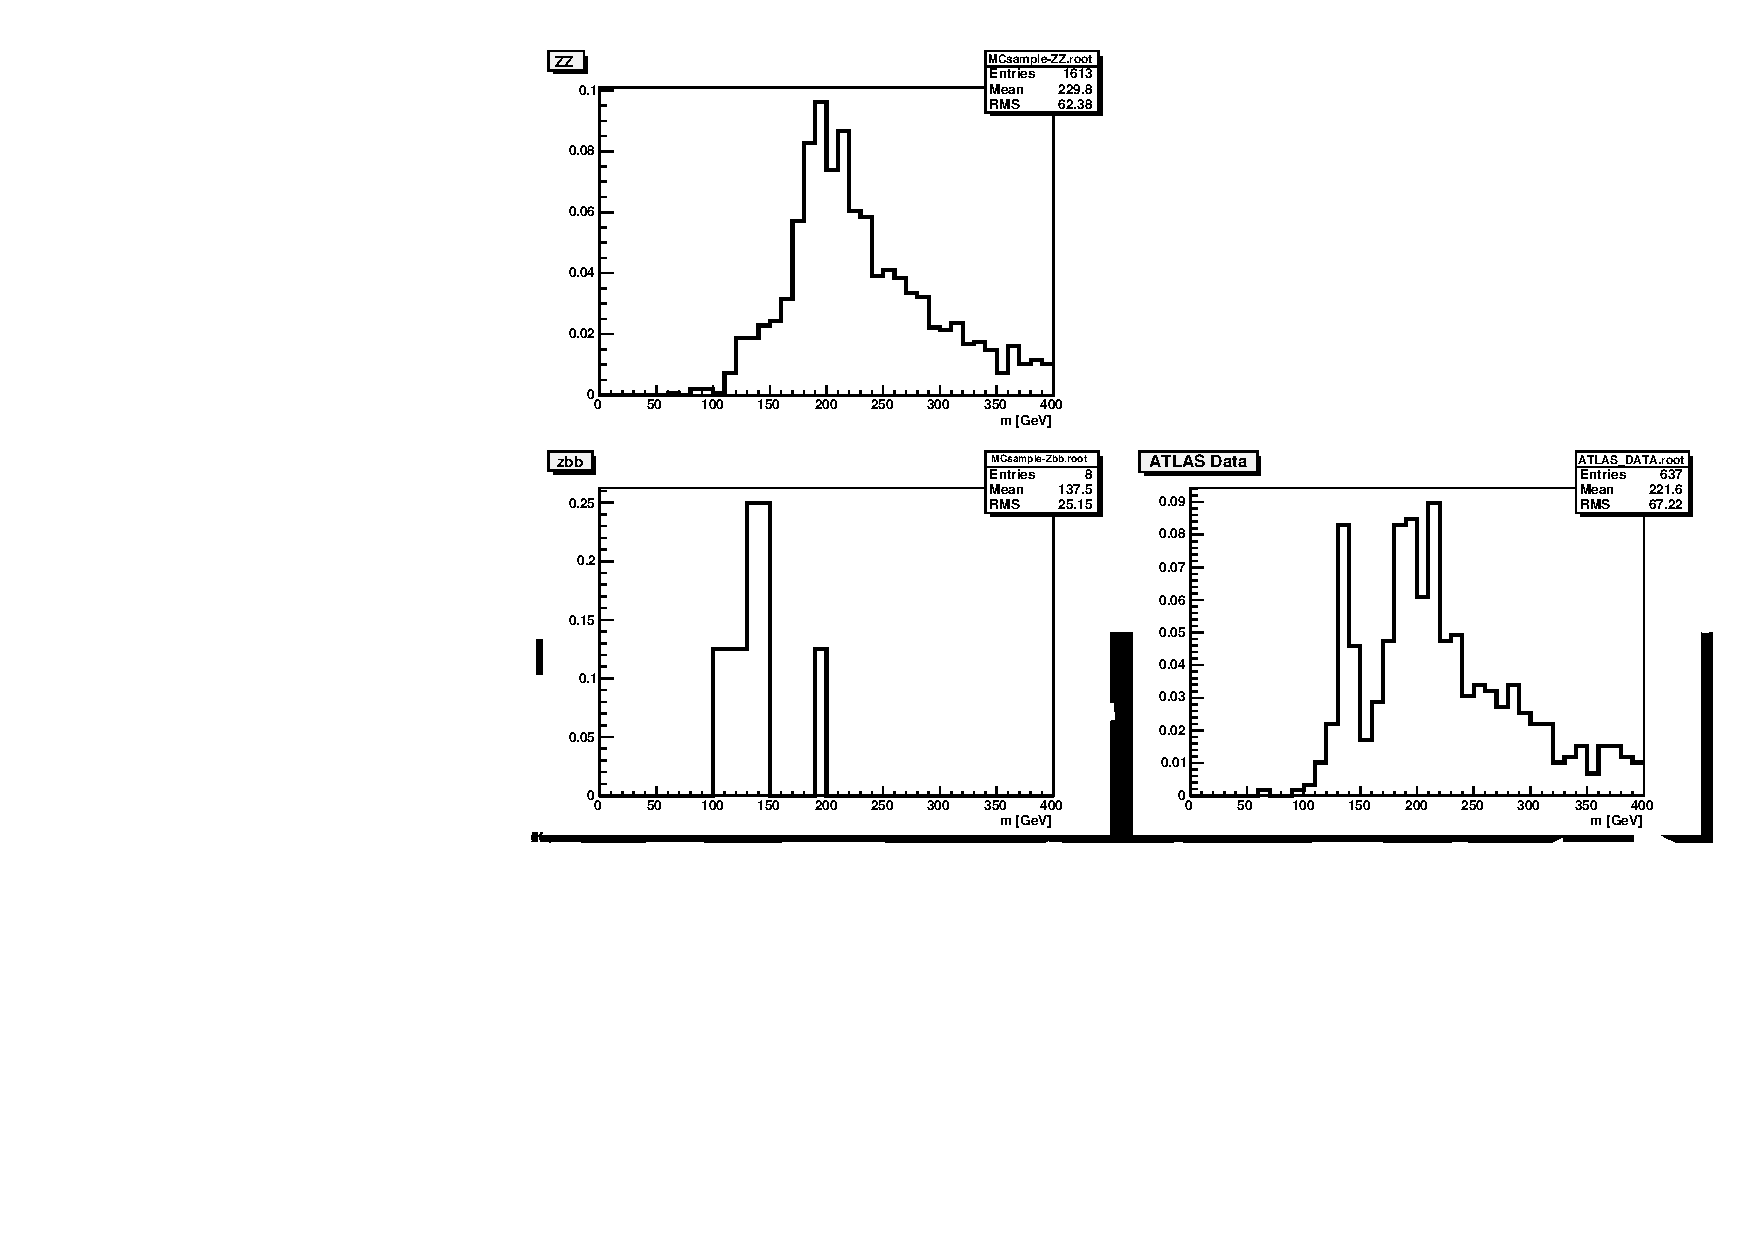
\includegraphics[width=0.8\textwidth]{ZZ/Higgs_mass_cut.pdf}
    \end{center}
    \caption{Invariant mass distribution of four leptons from different signal
    and background data. The mass peak at 125\;GeV in the ATLAS data is assumed to be the Higgs boson. }
    \label{fig:higgsmass}
\end{figure}


\section{Discussion}
\label{sec:discussion}

\subsection{Muon momentum loss}
The most surprising result from the muon momentum loss calculation was the fact
that of the 20 events, 8 events were observed where the muon actually seemed to
gain energy after passing through the electromagnetic calorimeter.This is
obviously highly unphysical. Unfortunately with only 20 events it is difficult
to pinpoint exactly which systematic or statistical errors have been made. One
possible explanation is that the tracker, which gets less precise with higher
energy failed to properly track the particles. However there seems no apparent
correlation between total energy and the momentum-gaining events.A more
probable solution would be the assumption that these events were not properly
reconstructed, for example because the particles might have flown partially
back into the beam axis, meaning the pseudorapidity is too high. Unfortunately
the pseudorapidity was not measured. From the literature, one expects an energy
loss of around 3\;GeV for muons with $p_T\approx100\;$GeV \cite{loss}, which
roughly fits with the calculated value when ignoring the energy-gain cases.

\subsection{Reconstruction of the $Z$ mass}
The $Z$ mass we obtained is smaller in all cases than the literature value.
Perhaps some energy was lost when selecting the calorimeter entries by hand.
However, a sample size of three gives hardly any ground to base this assumption
in. For the event $b)$, it is obvious that the inner detector failed to
properly track the particle. This is clear when comparing the energy scales of
both inner detector and calorimeter values. A possibility is again that the
pseudorapidity is too large, since it is close to the detector limit of
$\eta\leq2.5$ in this particular event. Possibly the calorimeter delivered a
better value since it has better coverage.

\subsection{ZZ selection}
in the selection of the $ZZ$ events a surprising amount of background could be
discarded by only two cut criteria. Overall, $74\%$ of the signal was
retrieved. Fortunately, the cut criteria here could be physically motivated in
the appearance of the hadrons, what probably resulted in the success.

\subsection{Analysis of the production threshold of ZZ pairs}
As expected, very few real ZZ pairs were observed below the production
threshold. Of course, theoretically we expect no events at all, since it should
be impossible to create a real ZZ pair below its production threshold.
However, the definition of ``real'' and ``virtual'' used here is not sharp.
Therefore, ZZ pairs that have a mass below the production threshold are
still counted as being real. It is furthermore apparent that ZZ$^*$ events are
the most likely. This can be explained by the fact that both the first or the
second Z can be virtual. Therefore, combinatorially, it has the most possible
configurations.\\
From the cut selection, 4561 ZZ pairs were found in the simulated data. At the
same luminosity, 3457 ZZ events were counted here. This is inconsistent with the
fact that it was required that two electrons and two muons were part of the
event and may be a hint at new physics in the mystery data.

\subsection{Search for new physics and Higgs boson}
As before, a decent selection was achieved with only two variable cuts. This may
be surprising since the search was an all-purpose search without any clear
indication what to look for. In practise it is way more fruitful to have a
physical understanding of models beyond the SM and what predictions they make
for different variables. Then, specific cuts can be employed to test, whether
these predictions are observed, or not. Still in one of the four mystery data
sets, a large amount of high-invariant-mass events was observed. Still, there
is no indication what type of new physics is observed, since virtually all
types of new particles are assumed to be at the higher mass-scale, since they
would have been found by now, otherwise.\\
The significance calculated here is to be taken as a rough estimate and not as
a proper $\sigma$-significance. Therefore, the unusual high significance of
26$\pm$1 has to be taken with a grain of salt.\\
For the Higgs search, a more modest significance of $2.6\pm1.1$ was found.
However, the peak is clearly visible in the data. At least a significance of 3
would be needed to claim a discovery. Most probably, time constraints were the
culprits here and clearer inspection of combinations of variable cuts could
probably have delivered a better result.

\subsection{Final comments}
This lab has been a good overview about both the theory behind the Standard
Model as well as the experimental and statistical methods employed to analyse
particle collision experiments. That being said, it lacks a bit of focus. It
was initially assumed that the main part of this experiment was the detection
and analysis of the Higgs boson, however, this proofed to be a small side-task.
\\Having a way to visually represent different particle combinations in
ATLANTIS has been pedagogically useful as a means to gain some intuition on the
matter. However, it has to be clear that there is no actual usage of this tool
in real experimental analysis.
Still, the experiment is recommended for those eager to understand the
properties of the Higgs boson and the Standard Model in general.


\bibliography{literatur}
\end{document}

